\documentclass[11pt]{report}

% Packages nécessaires
\usepackage[utf8]{inputenc}
\usepackage[T1]{fontenc}
\usepackage[french]{babel}
\usepackage{graphicx}
\usepackage{amsmath}
\usepackage{amssymb}
\usepackage{hyperref}
\usepackage{booktabs}
\usepackage{xcolor}
\usepackage{fancyhdr}
\usepackage{geometry}
\usepackage{float}
\usepackage{caption}
\usepackage{subcaption}
\usepackage{titlesec}

% Configuration de la géométrie de la page
\geometry{margin=2.5cm}

% Configuration des liens hypertexte
\hypersetup{
    colorlinks=true,
    linkcolor=blue,
    filecolor=magenta,      
    urlcolor=cyan,
    pdftitle={Analyse Financière avec Data Science et Machine Learning},
    pdfauthor={Équipe GE Finance},
    pdfsubject={Rapport d'analyse},
    pdfkeywords={finance, data science, machine learning}
}

% Configuration des en-têtes et pieds de page
\pagestyle{fancy}
\fancyhf{}
\fancyhead[L]{\textit{Analyse Financière}}
\fancyhead[R]{\thepage}
\fancyfoot[C]{\textit{Projet GE - 2025}}

% Configuration des titres
\titleformat{\chapter}[display]
{\normalfont\huge\bfseries}{\chaptertitlename\ \thechapter}{20pt}{\Huge}
\titlespacing*{\chapter}{0pt}{50pt}{40pt}

% Titre principal
\title{
    \vspace{-2cm}
    
\includegraphics[width=0.3\textwidth]{figures/logo-ecc.png}\\[1cm]
    \LARGE{École Centrale Casablanca}\\[0.5cm]
    \rule{\linewidth}{0.5mm}\\[0.4cm]
    \huge{\textbf{Analyse Financière avec\\Data Science \& Machine Learning}}\\
    \rule{\linewidth}{0.5mm}\\[1.5cm]
}

\author{
    \large
    \textbf{Auteurs:}\\
    Salah Eddine EL AZOUTI\\
    Salma Saaidi\\
    Anas EL HAYEL\\
    Walid EL BOUCHTI\\
    Aasma ouamalich
}

\date{\today}

\begin{document}

\maketitle
\thispagestyle{empty}

\newpage
\tableofcontents
\thispagestyle{empty}

\newpage
\chapter*{Résumé}
\addcontentsline{toc}{chapter}{Résumé}
Ce projet porte sur l'analyse financière approfondie d'entreprises américaines à l'aide de techniques de Data Science et de Machine Learning. À partir d'un jeu de données contenant 200 indicateurs financiers d'entreprises américaines entre 2014 et 2018, nous avons réalisé une exploration complète, calculé des ratios financiers, identifié des clusters d'entreprises aux profils similaires, construit des modèles prédictifs et interprété les résultats d'un point de vue économique.

Le présent rapport détaille la méthodologie utilisée, les résultats obtenus et les conclusions économiques tirées de cette analyse. Ce travail démontre comment les techniques modernes d'analyse de données peuvent être appliquées au domaine financier pour extraire des informations pertinentes et actionables.

\chapter{Introduction}
\section{Contexte}
L'analyse financière traditionnelle repose sur l'examen manuel d'un nombre limité de ratios et d'indicateurs financiers. Avec l'avènement du Big Data et de l'intelligence artificielle, il est désormais possible d'analyser simultanément des centaines d'indicateurs et d'identifier des motifs que l'œil humain ne pourrait discerner. 

Ce projet s'inscrit dans cette démarche en proposant une analyse financière augmentée par des techniques de Data Science et de Machine Learning. L'objectif est d'exploiter la puissance de ces outils pour extraire des insights précieux à partir d'un vaste ensemble de données financières.

\section{Objectifs}
Les principaux objectifs de ce projet sont les suivants :
\begin{itemize}
    \item Explorer et nettoyer un dataset contenant 200 indicateurs financiers d'entreprises américaines
    \item Calculer et analyser des ratios financiers clés (ROA, ROE, marge nette, etc.)
    \item Identifier des groupes d'entreprises aux profils financiers similaires à l'aide de techniques de clustering
    \item Construire des modèles prédictifs pour anticiper les performances financières
    \item Interpréter les résultats d'un point de vue économique et financier
    \item Proposer des recommandations stratégiques basées sur l'analyse
\end{itemize}

\section{Structure du rapport}
Ce rapport est structuré comme suit :
\begin{itemize}
    \item \textbf{Chapitre 2} : Présentation du jeu de données et exploration initiale
    \item \textbf{Chapitre 3} : Calcul et visualisation des ratios financiers
    \item \textbf{Chapitre 4} : Analyse en composantes principales et clustering
    \item \textbf{Chapitre 5} : Modélisation prédictive
    \item \textbf{Chapitre 6} : Conclusions et interprétations économiques
\end{itemize}

\chapter{Données et exploration initiale}
\section{Présentation du jeu de données}
Le jeu de données utilisé dans ce projet contient 200 indicateurs financiers pour un ensemble d'entreprises américaines cotées en bourse sur la période 2014-2018. Ces indicateurs couvrent divers aspects de la performance financière, notamment :
\begin{itemize}
    \item Informations générales (nom de l'entreprise, secteur, etc.)
    \item Métriques de revenus et de profits
    \item Informations sur les actifs et les passifs
    \item Indicateurs de performance boursière
\end{itemize}

\section{Exploration des données}
\subsection{Structure générale}
L'exploration initiale des données nous a permis de comprendre la structure générale du jeu de données, notamment le nombre d'entreprises, la distribution par secteur et les statistiques descriptives des principaux indicateurs financiers.

\begin{figure}[H]
    \centering
    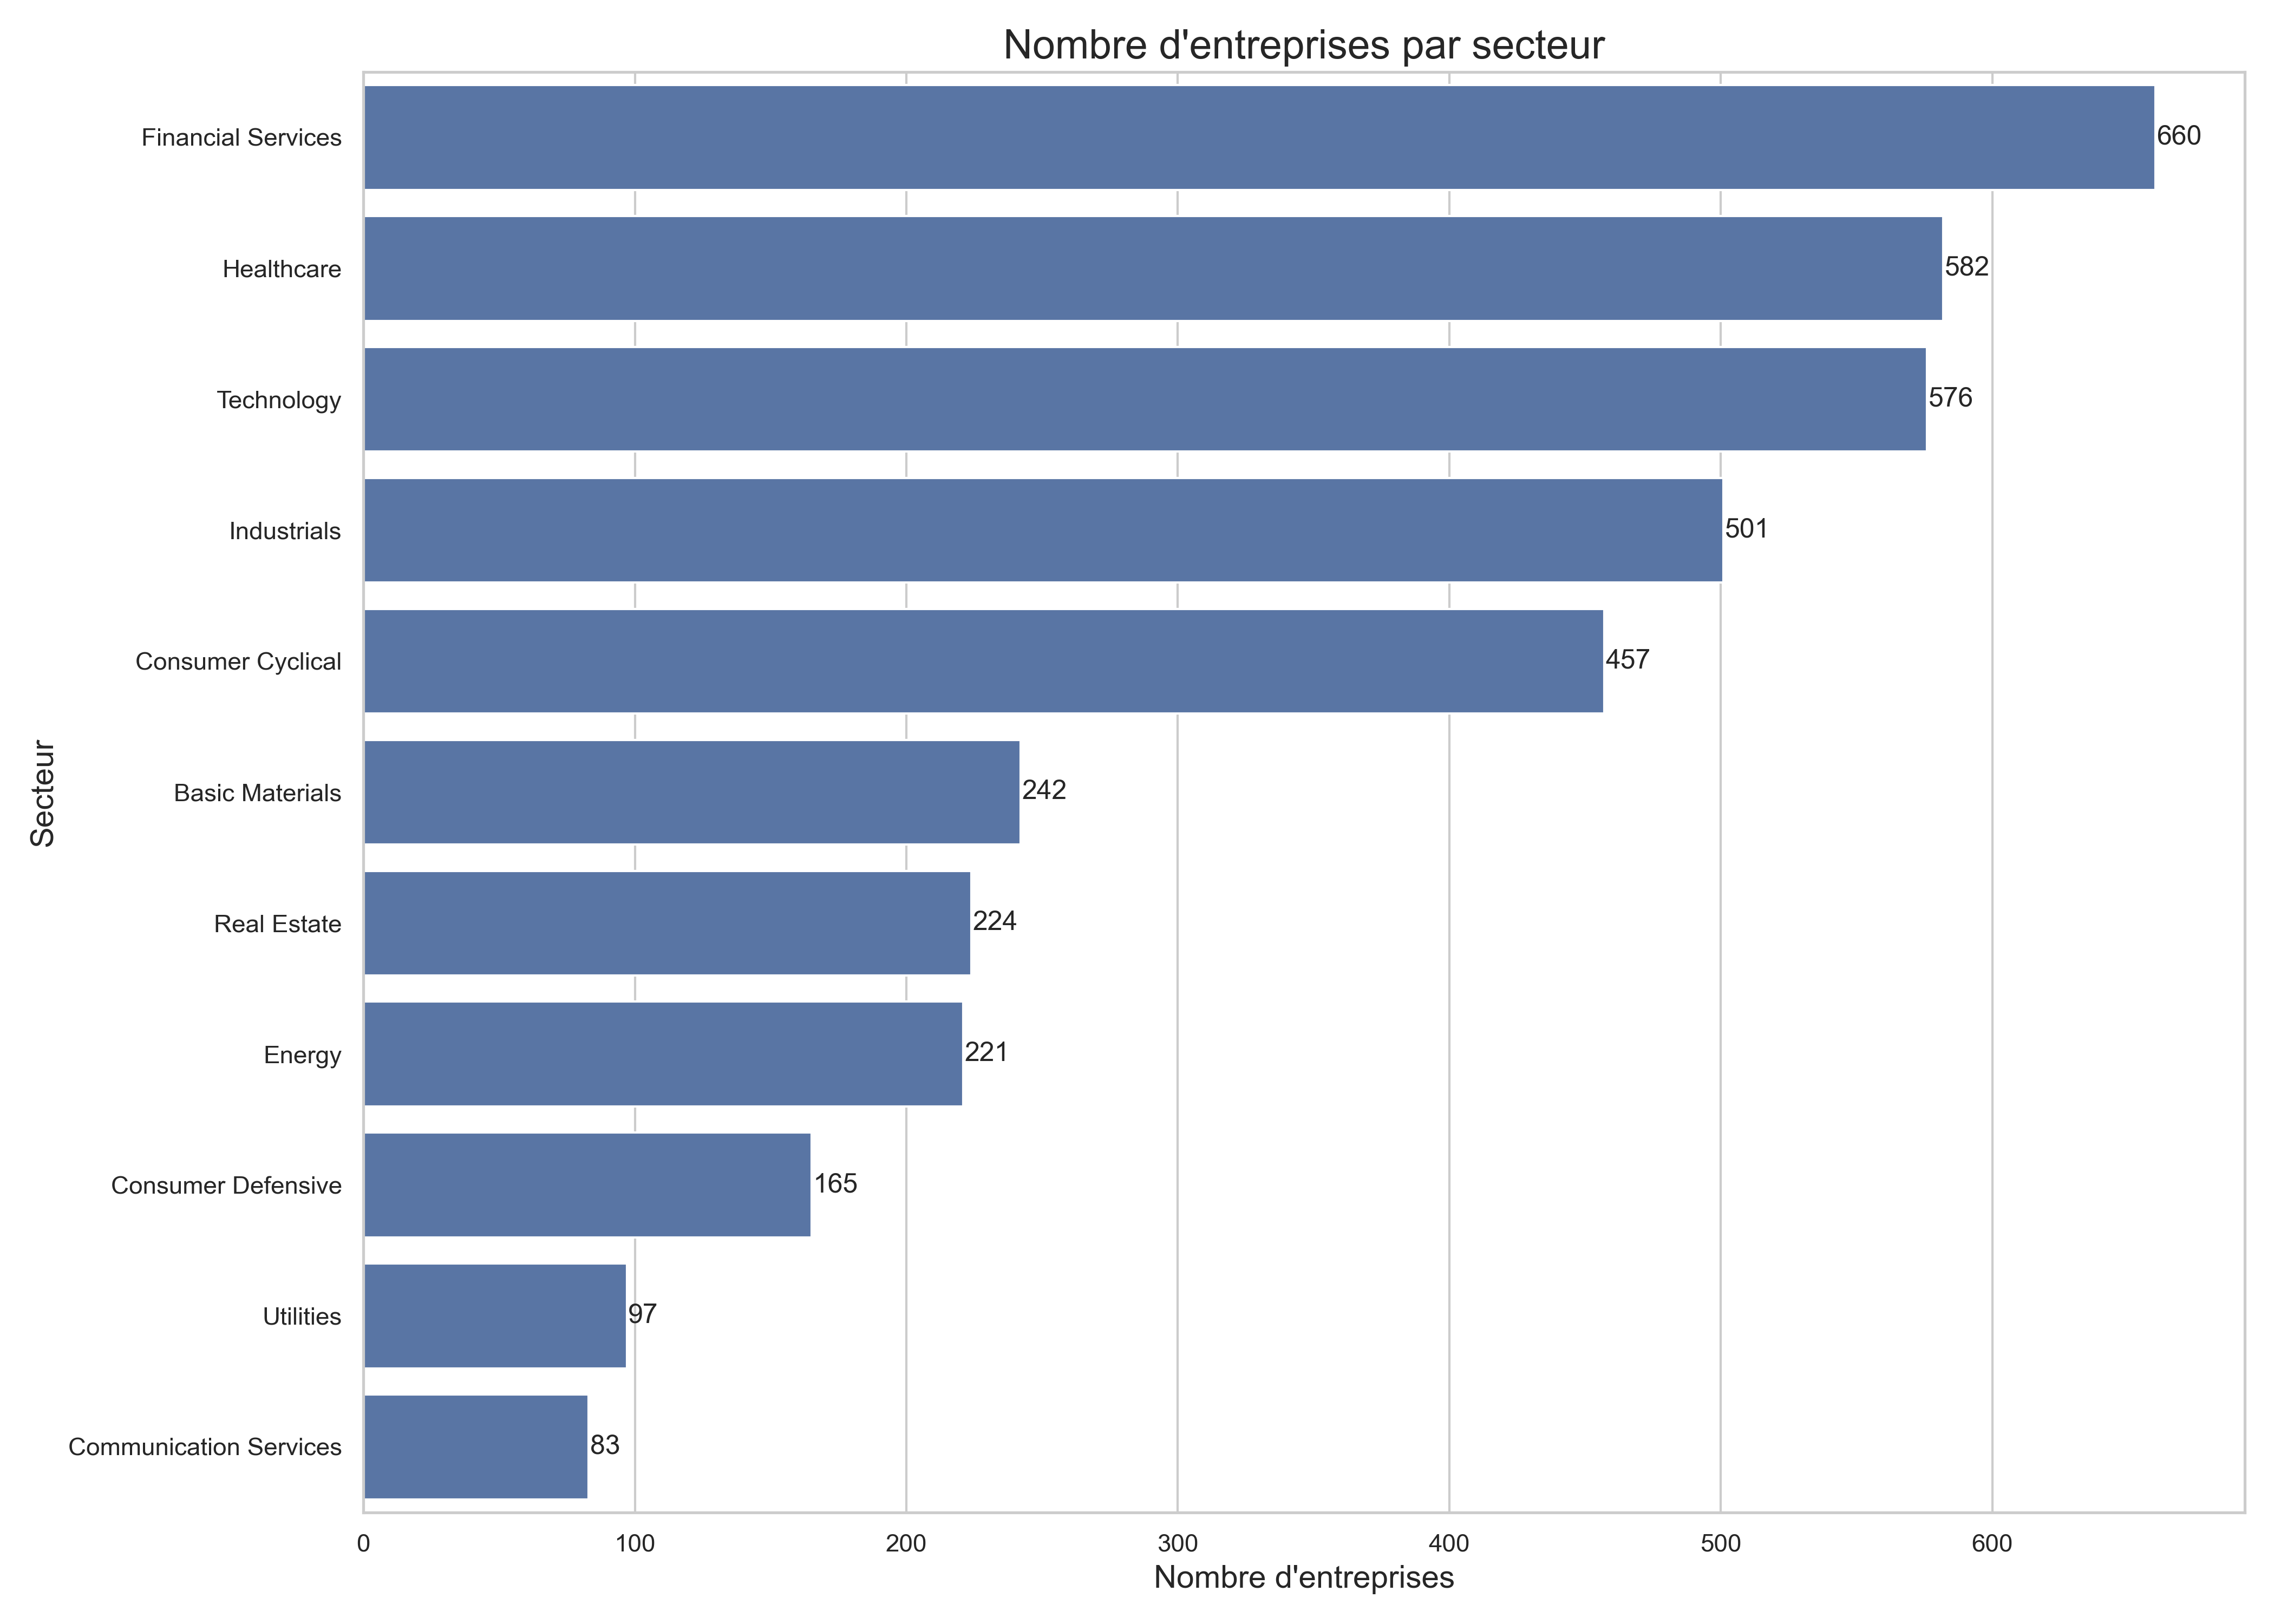
\includegraphics[width=0.9\textwidth]{figures/companies_by_sector.png}
    \caption{Distribution des entreprises par secteur}
    \label{fig:sector_distribution}
\end{figure}

La figure \ref{fig:sector_distribution} montre la répartition des entreprises par secteur dans notre jeu de données. On constate que certains secteurs sont plus représentés que d'autres, ce qui est important à prendre en compte lors de l'interprétation des résultats d'analyse.

\subsection{Traitement des valeurs manquantes}
L'analyse des valeurs manquantes est une étape cruciale dans la préparation des données pour l'analyse. Nous avons identifié les colonnes présentant des valeurs manquantes et appliqué des stratégies appropriées pour les traiter.

\subsection{Détection et traitement des valeurs aberrantes}
Les valeurs aberrantes peuvent fortement influencer les résultats des analyses statistiques et des modèles de machine learning. Nous avons mis en place des méthodes pour les détecter et les traiter de manière appropriée.

\chapter{Ratios financiers et visualisations}
\section{Calcul des ratios financiers}
Nous avons calculé plusieurs ratios financiers clés pour enrichir notre analyse :
\begin{itemize}
    \item \textbf{ROA (Return on Assets)} : Mesure la rentabilité des actifs
    \item \textbf{ROE (Return on Equity)} : Mesure la rentabilité des capitaux propres
    \item \textbf{Marge nette} : Rapport entre le bénéfice net et le chiffre d'affaires
    \item \textbf{Ratio d'endettement} : Mesure du niveau d'endettement par rapport aux actifs
    \item \textbf{Ratio de liquidité} : Capacité à honorer les dettes à court terme
\end{itemize}

\section{Analyse des performances par secteur}
La performance financière varie considérablement selon les secteurs d'activité. Nous avons analysé comment les différents indicateurs et ratios se comportent à travers les divers secteurs représentés dans notre jeu de données.

\begin{figure}[H]
    \centering
    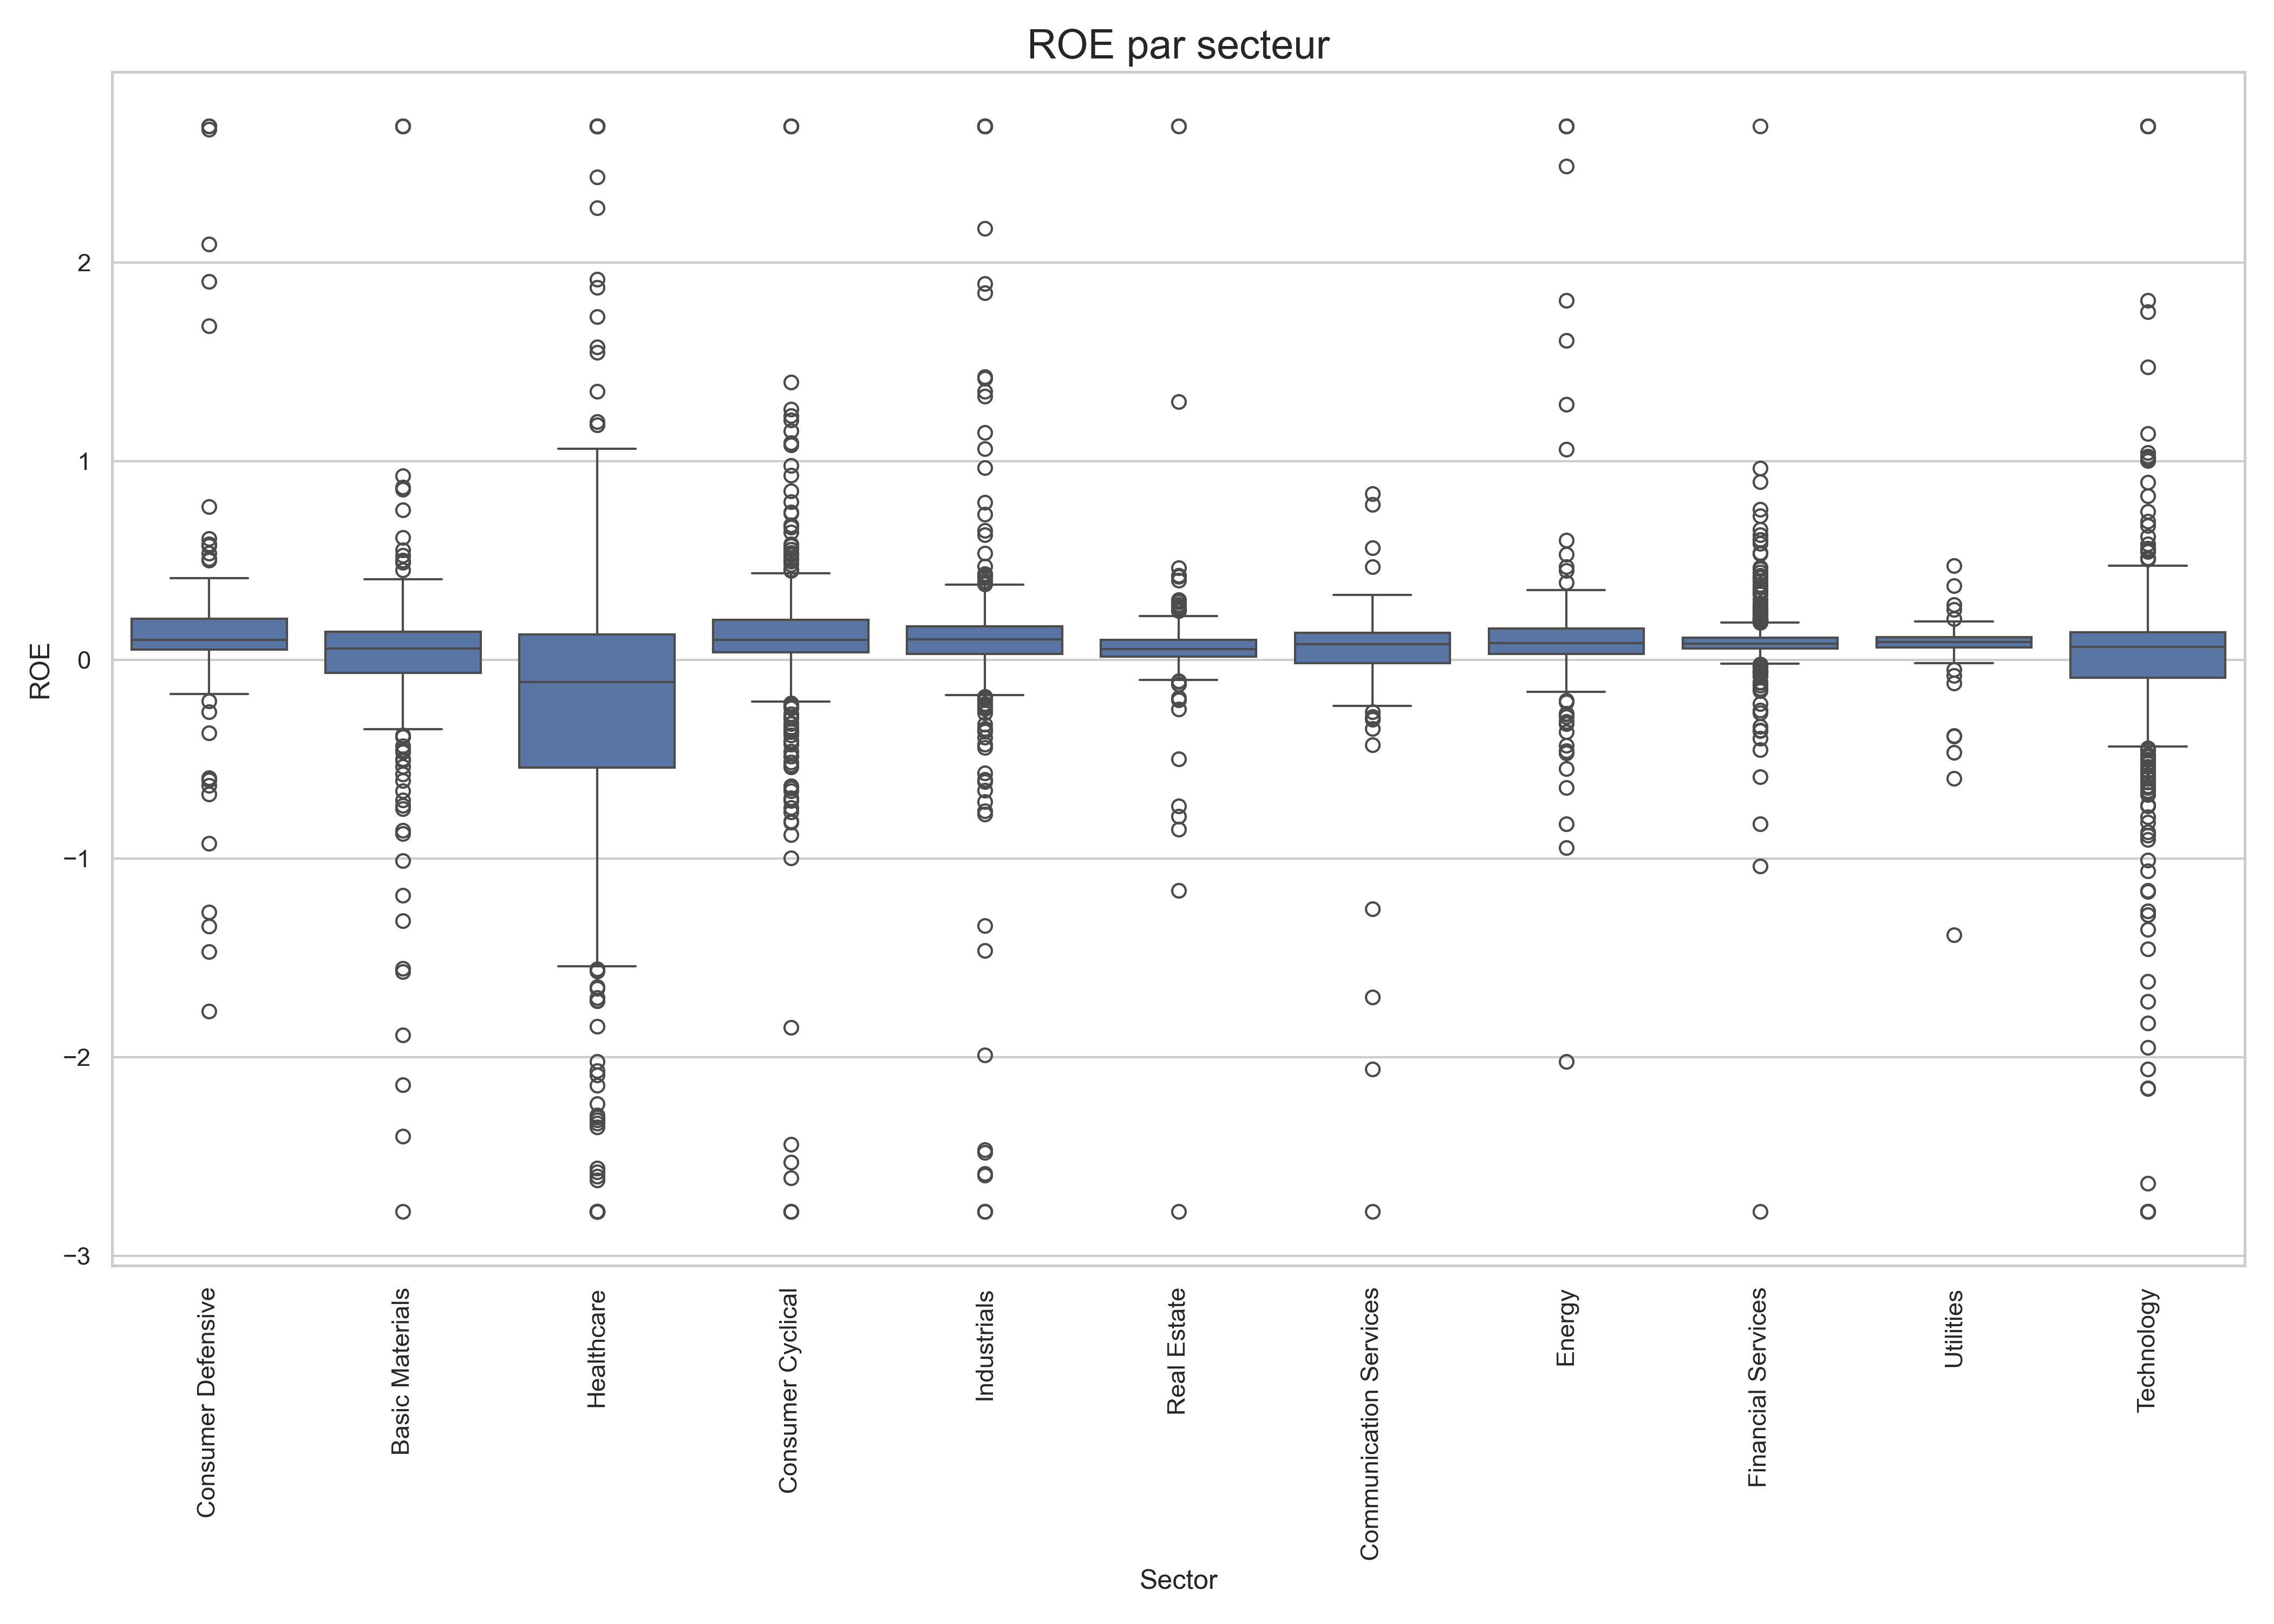
\includegraphics[width=0.9\textwidth]{figures/ROE_by_sector.png}
    \caption{Rentabilité des capitaux propres (ROE) par secteur}
    \label{fig:roe_by_sector}
\end{figure}

\begin{figure}[H]
    \centering
    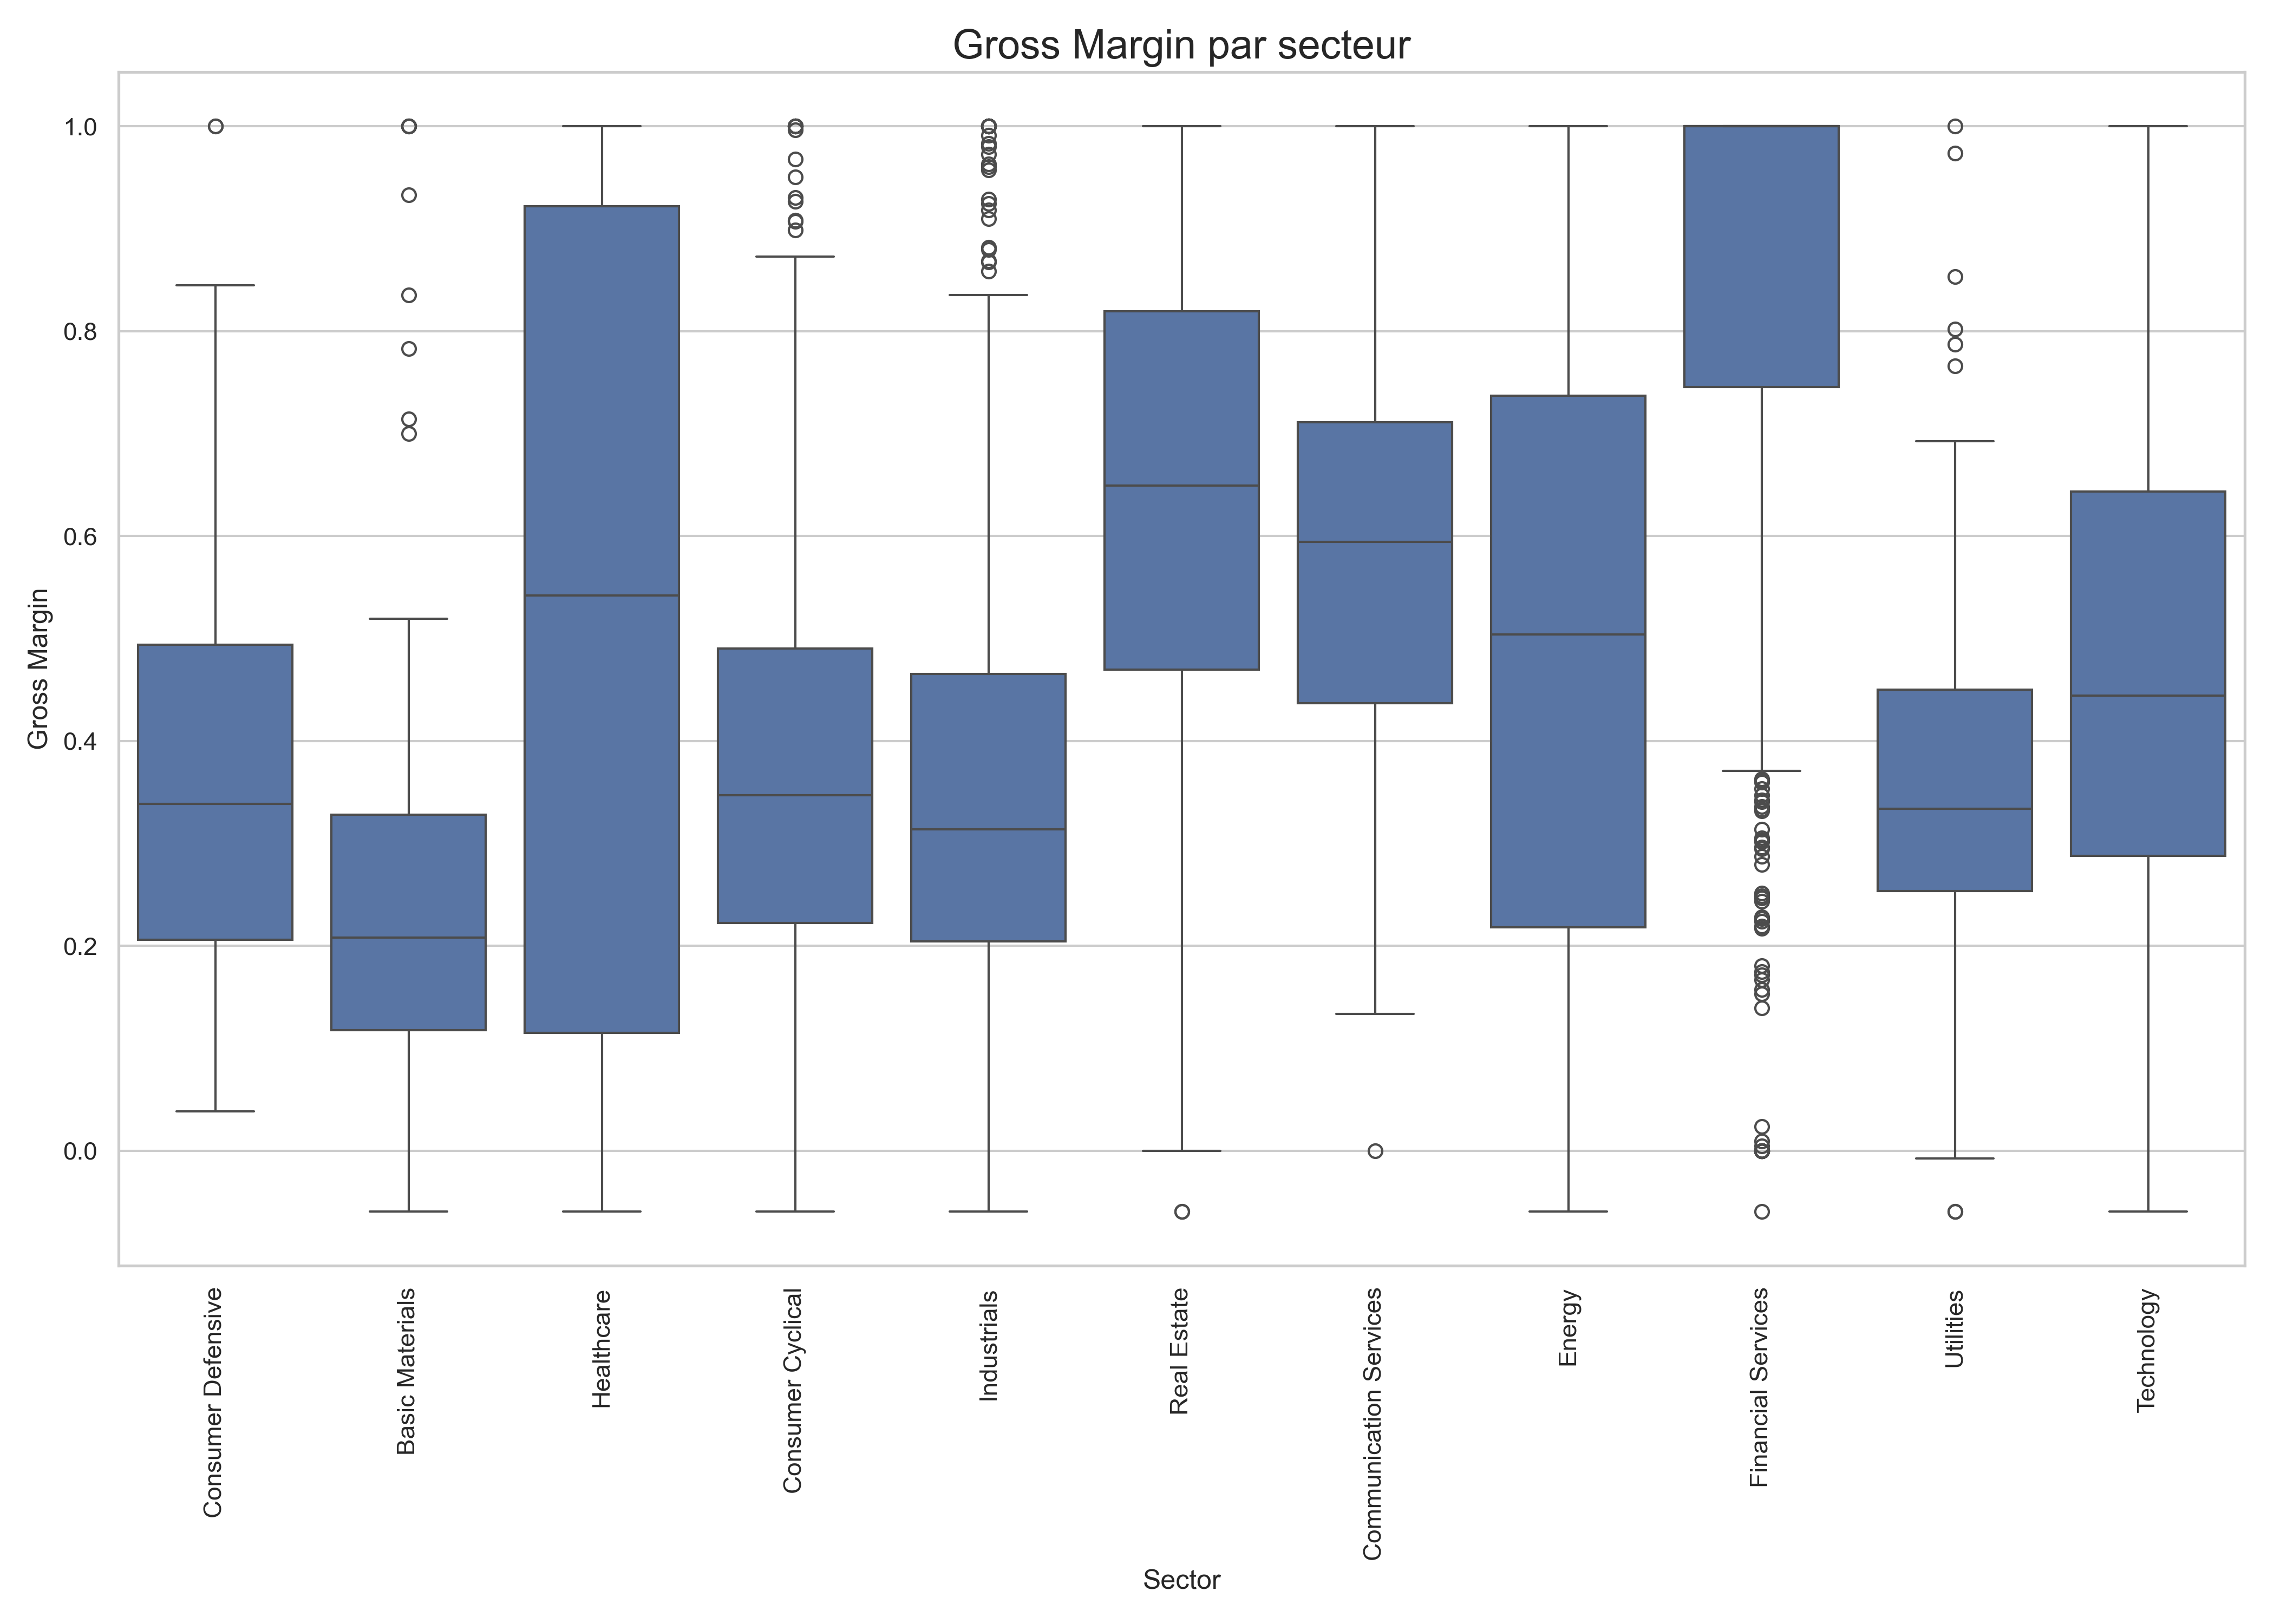
\includegraphics[width=0.9\textwidth]{figures/Gross_Margin_by_sector.png}
    \caption{Marge brute par secteur}
    \label{fig:gross_margin_by_sector}
\end{figure}

\begin{figure}[H]
    \centering
    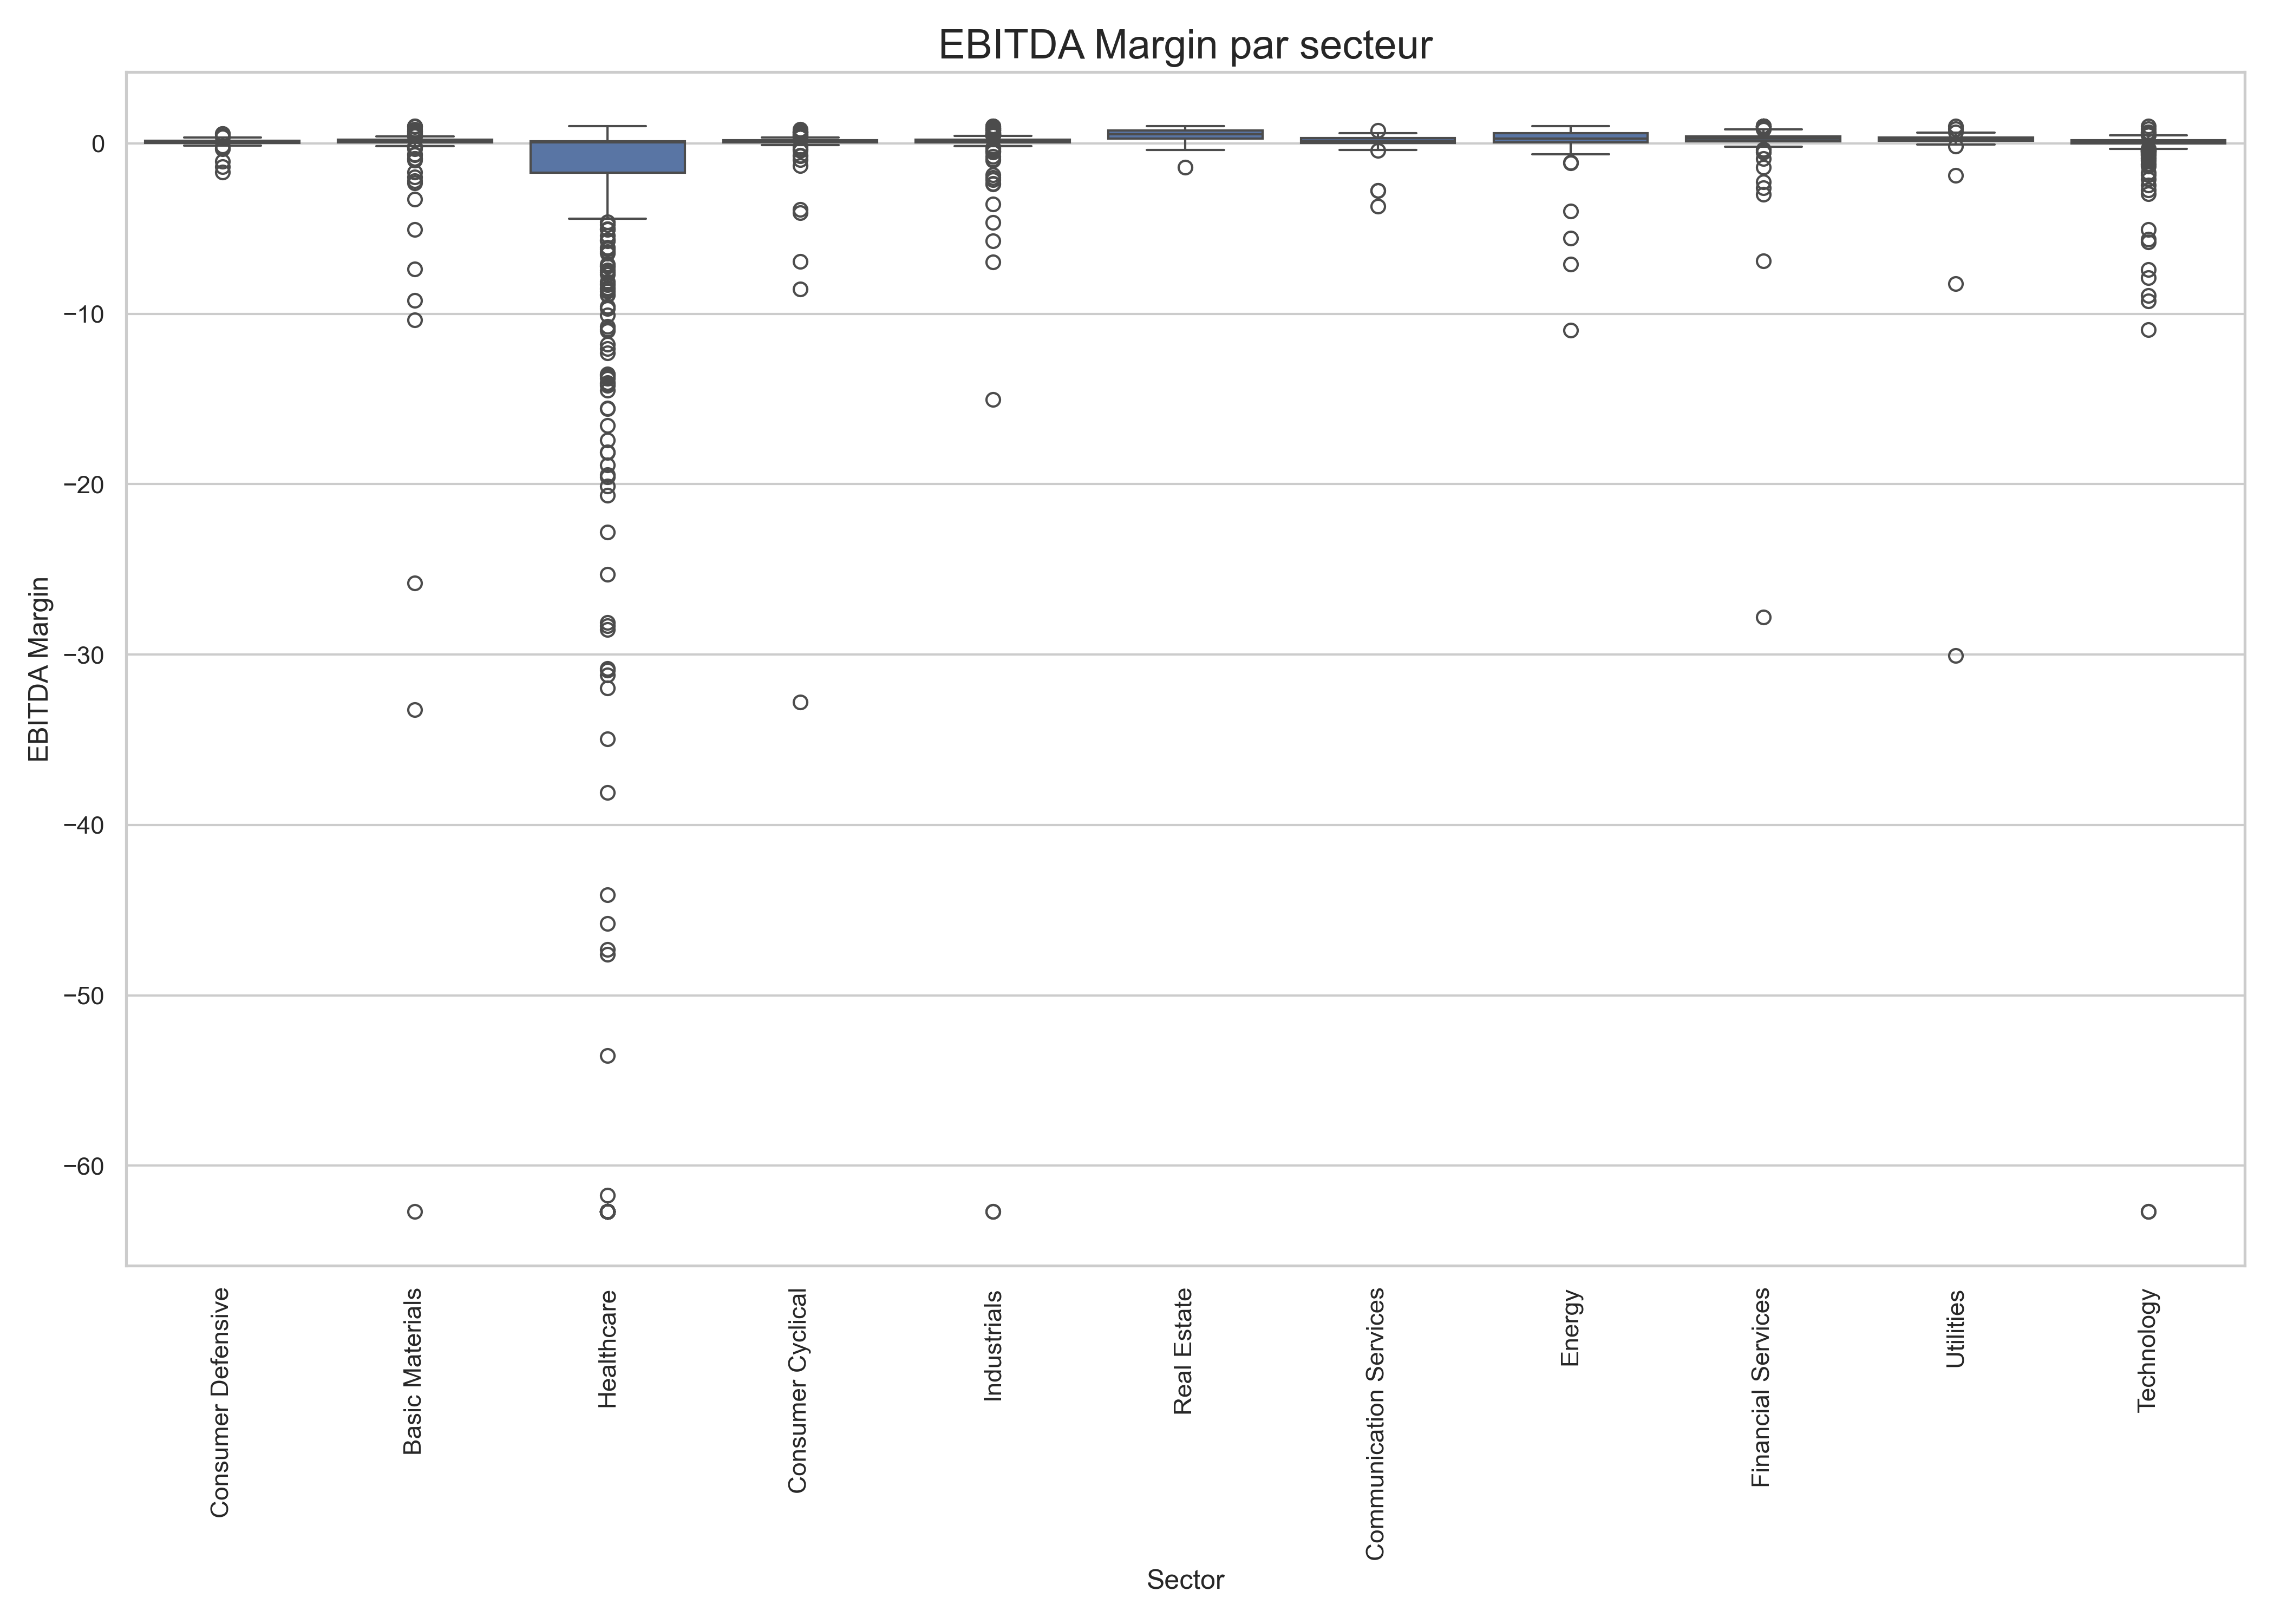
\includegraphics[width=0.9\textwidth]{figures/EBITDA_Margin_by_sector.png}
    \caption{Marge EBITDA par secteur}
    \label{fig:ebitda_margin_by_sector}
\end{figure}

Ces visualisations (figures \ref{fig:roe_by_sector}, \ref{fig:gross_margin_by_sector} et \ref{fig:ebitda_margin_by_sector}) mettent en évidence les différences significatives de performance financière entre les secteurs. On observe notamment que certains secteurs présentent des ratios de rentabilité plus élevés et plus stables que d'autres, ce qui peut être attribué à diverses caractéristiques sectorielles telles que les barrières à l'entrée, l'intensité concurrentielle et les structures de coûts.

\section{Corrélation entre variables financières}
L'étude des corrélations entre les différentes variables financières permet d'identifier des relations potentiellement significatives et d'orienter la suite de l'analyse.

\begin{figure}[H]
    \centering
    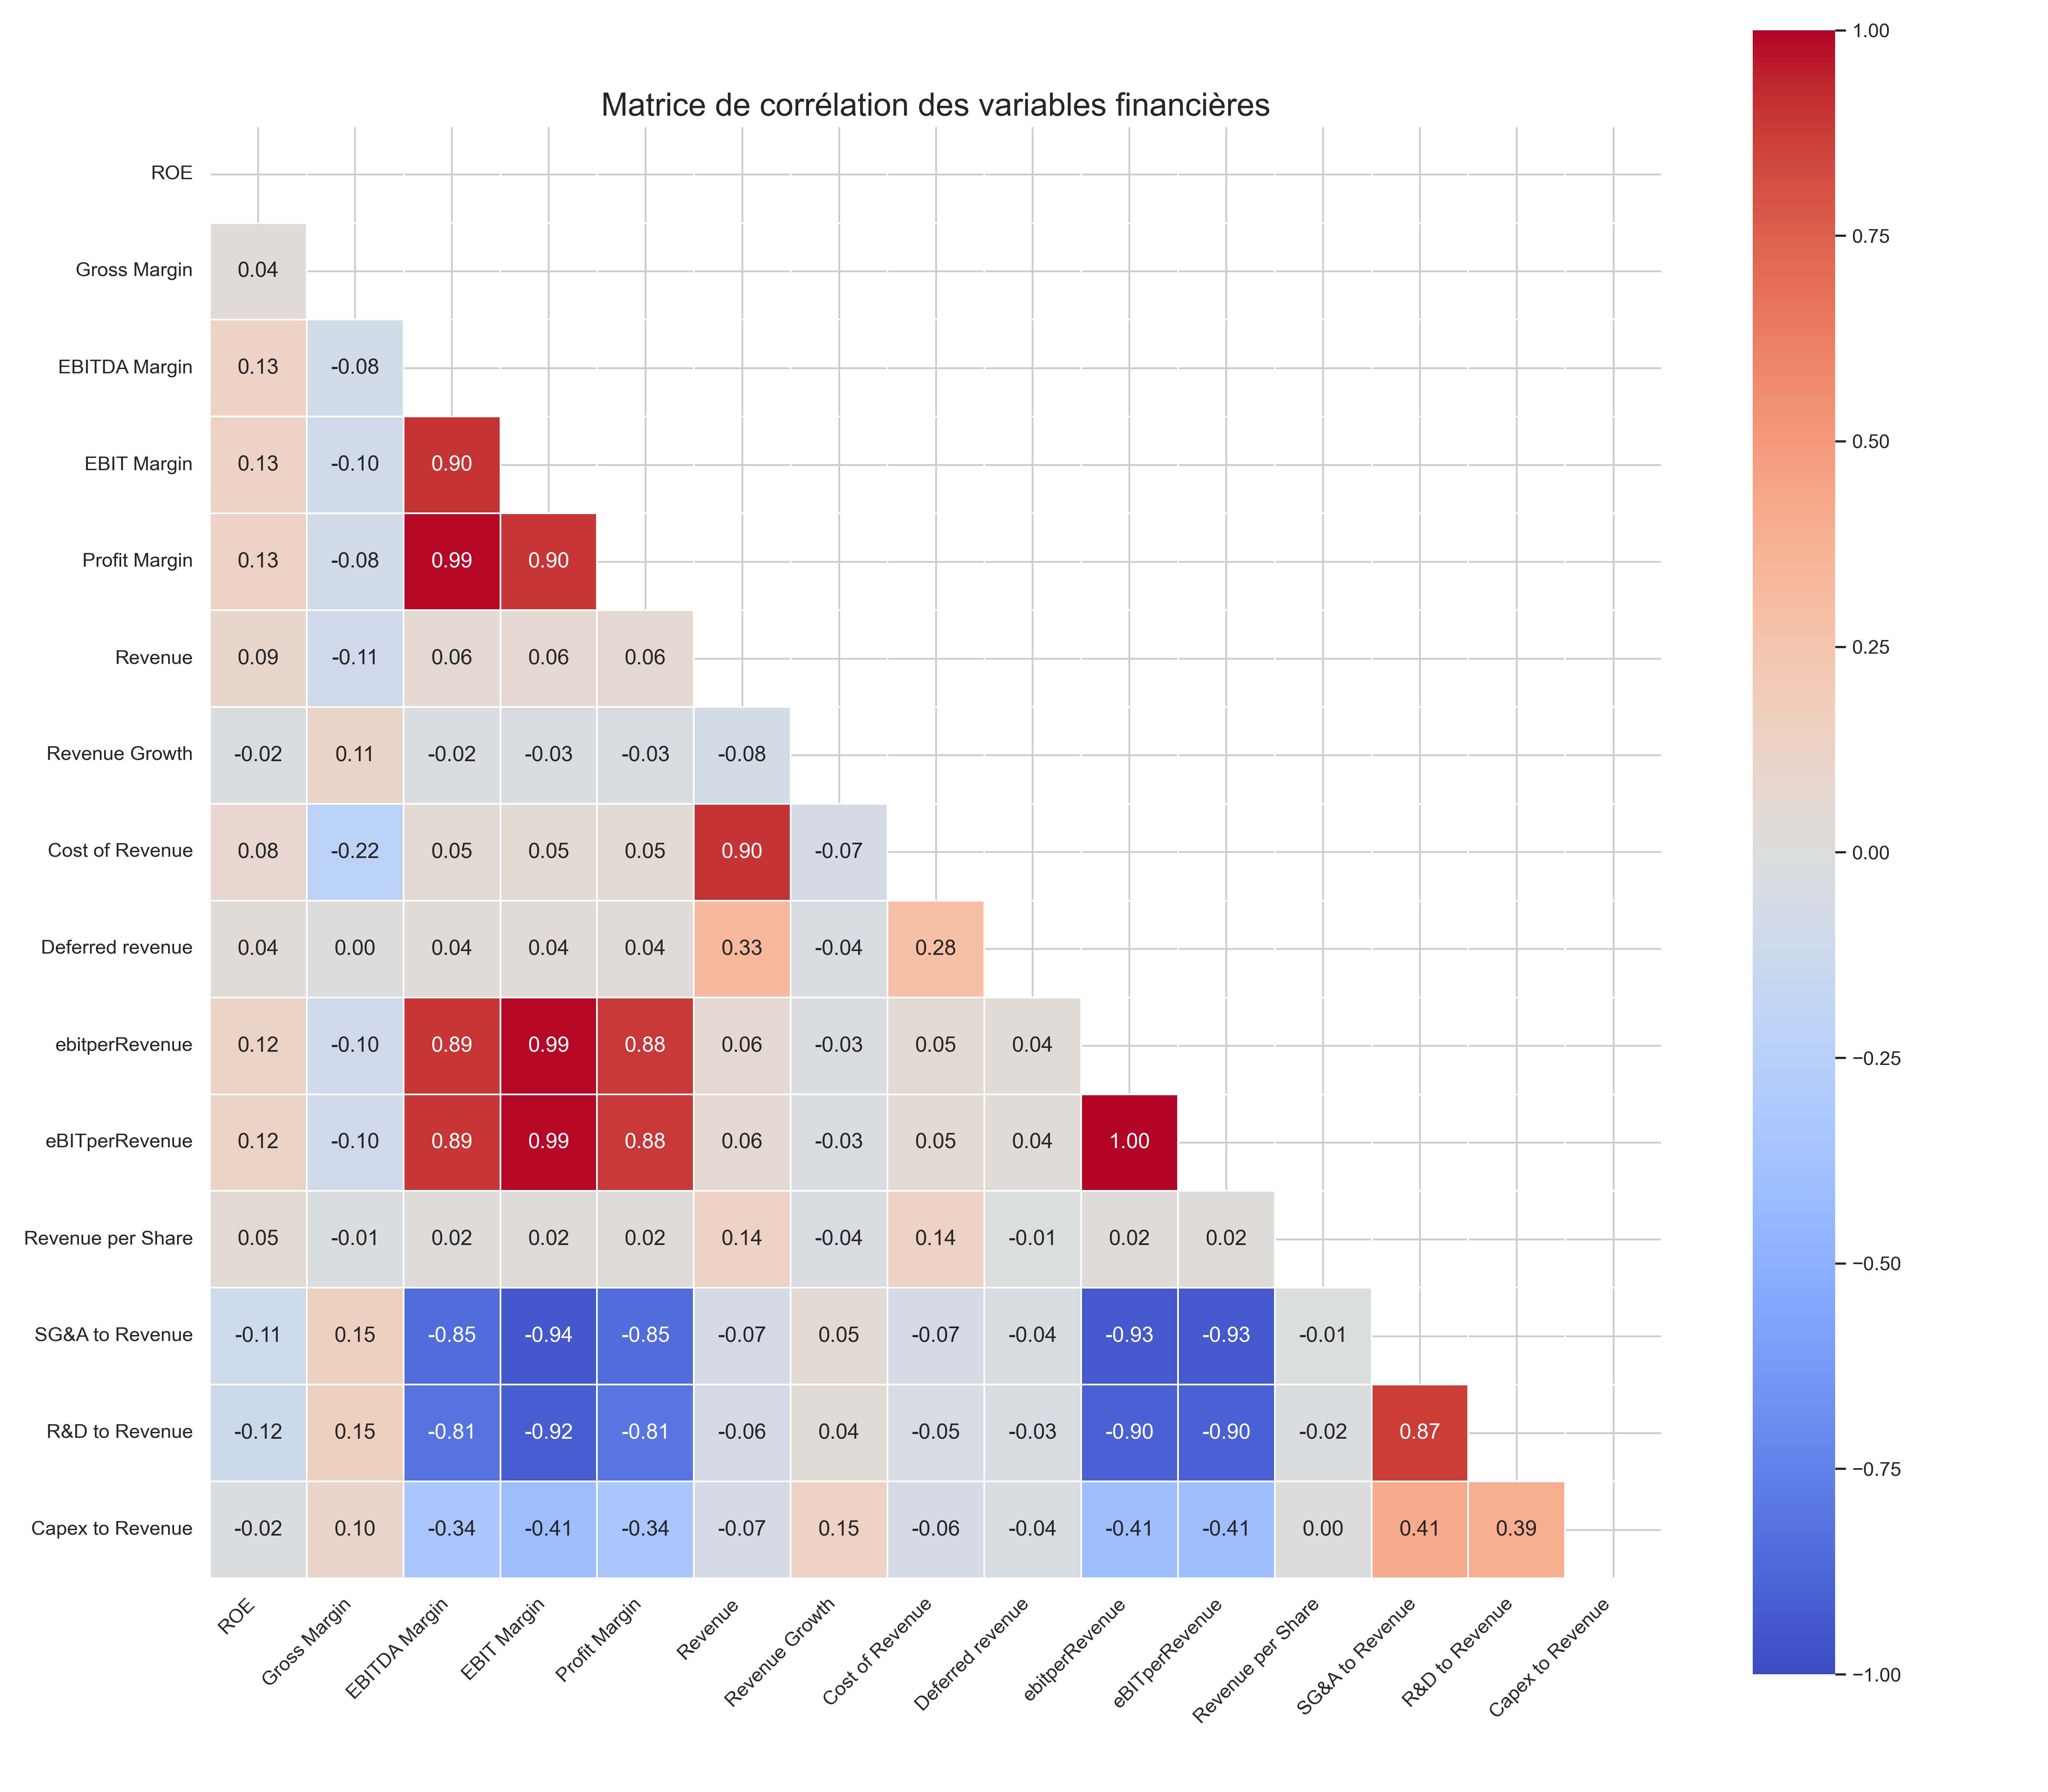
\includegraphics[width=0.95\textwidth]{figures/correlation_matrix.png}
    \caption{Matrice de corrélation des principales variables financières}
    \label{fig:correlation_matrix}
\end{figure}

La matrice de corrélation (figure \ref{fig:correlation_matrix}) révèle plusieurs relations importantes entre les variables financières. Les corrélations positives fortes (en bleu foncé) indiquent des variables qui évoluent généralement dans le même sens, tandis que les corrélations négatives (en rouge) montrent des variables qui tendent à évoluer en sens inverse. Ces informations sont cruciales pour comprendre les interactions entre différents aspects de la performance financière des entreprises.

\chapter{Analyse en composantes principales et clustering}
\section{Réduction de dimension par ACP}
L'Analyse en Composantes Principales (ACP) est une technique statistique puissante qui permet de réduire la dimensionnalité d'un jeu de données tout en conservant le maximum d'information. Nous l'avons appliquée à notre ensemble de données pour identifier les principales sources de variance.

\begin{figure}[H]
    \centering
    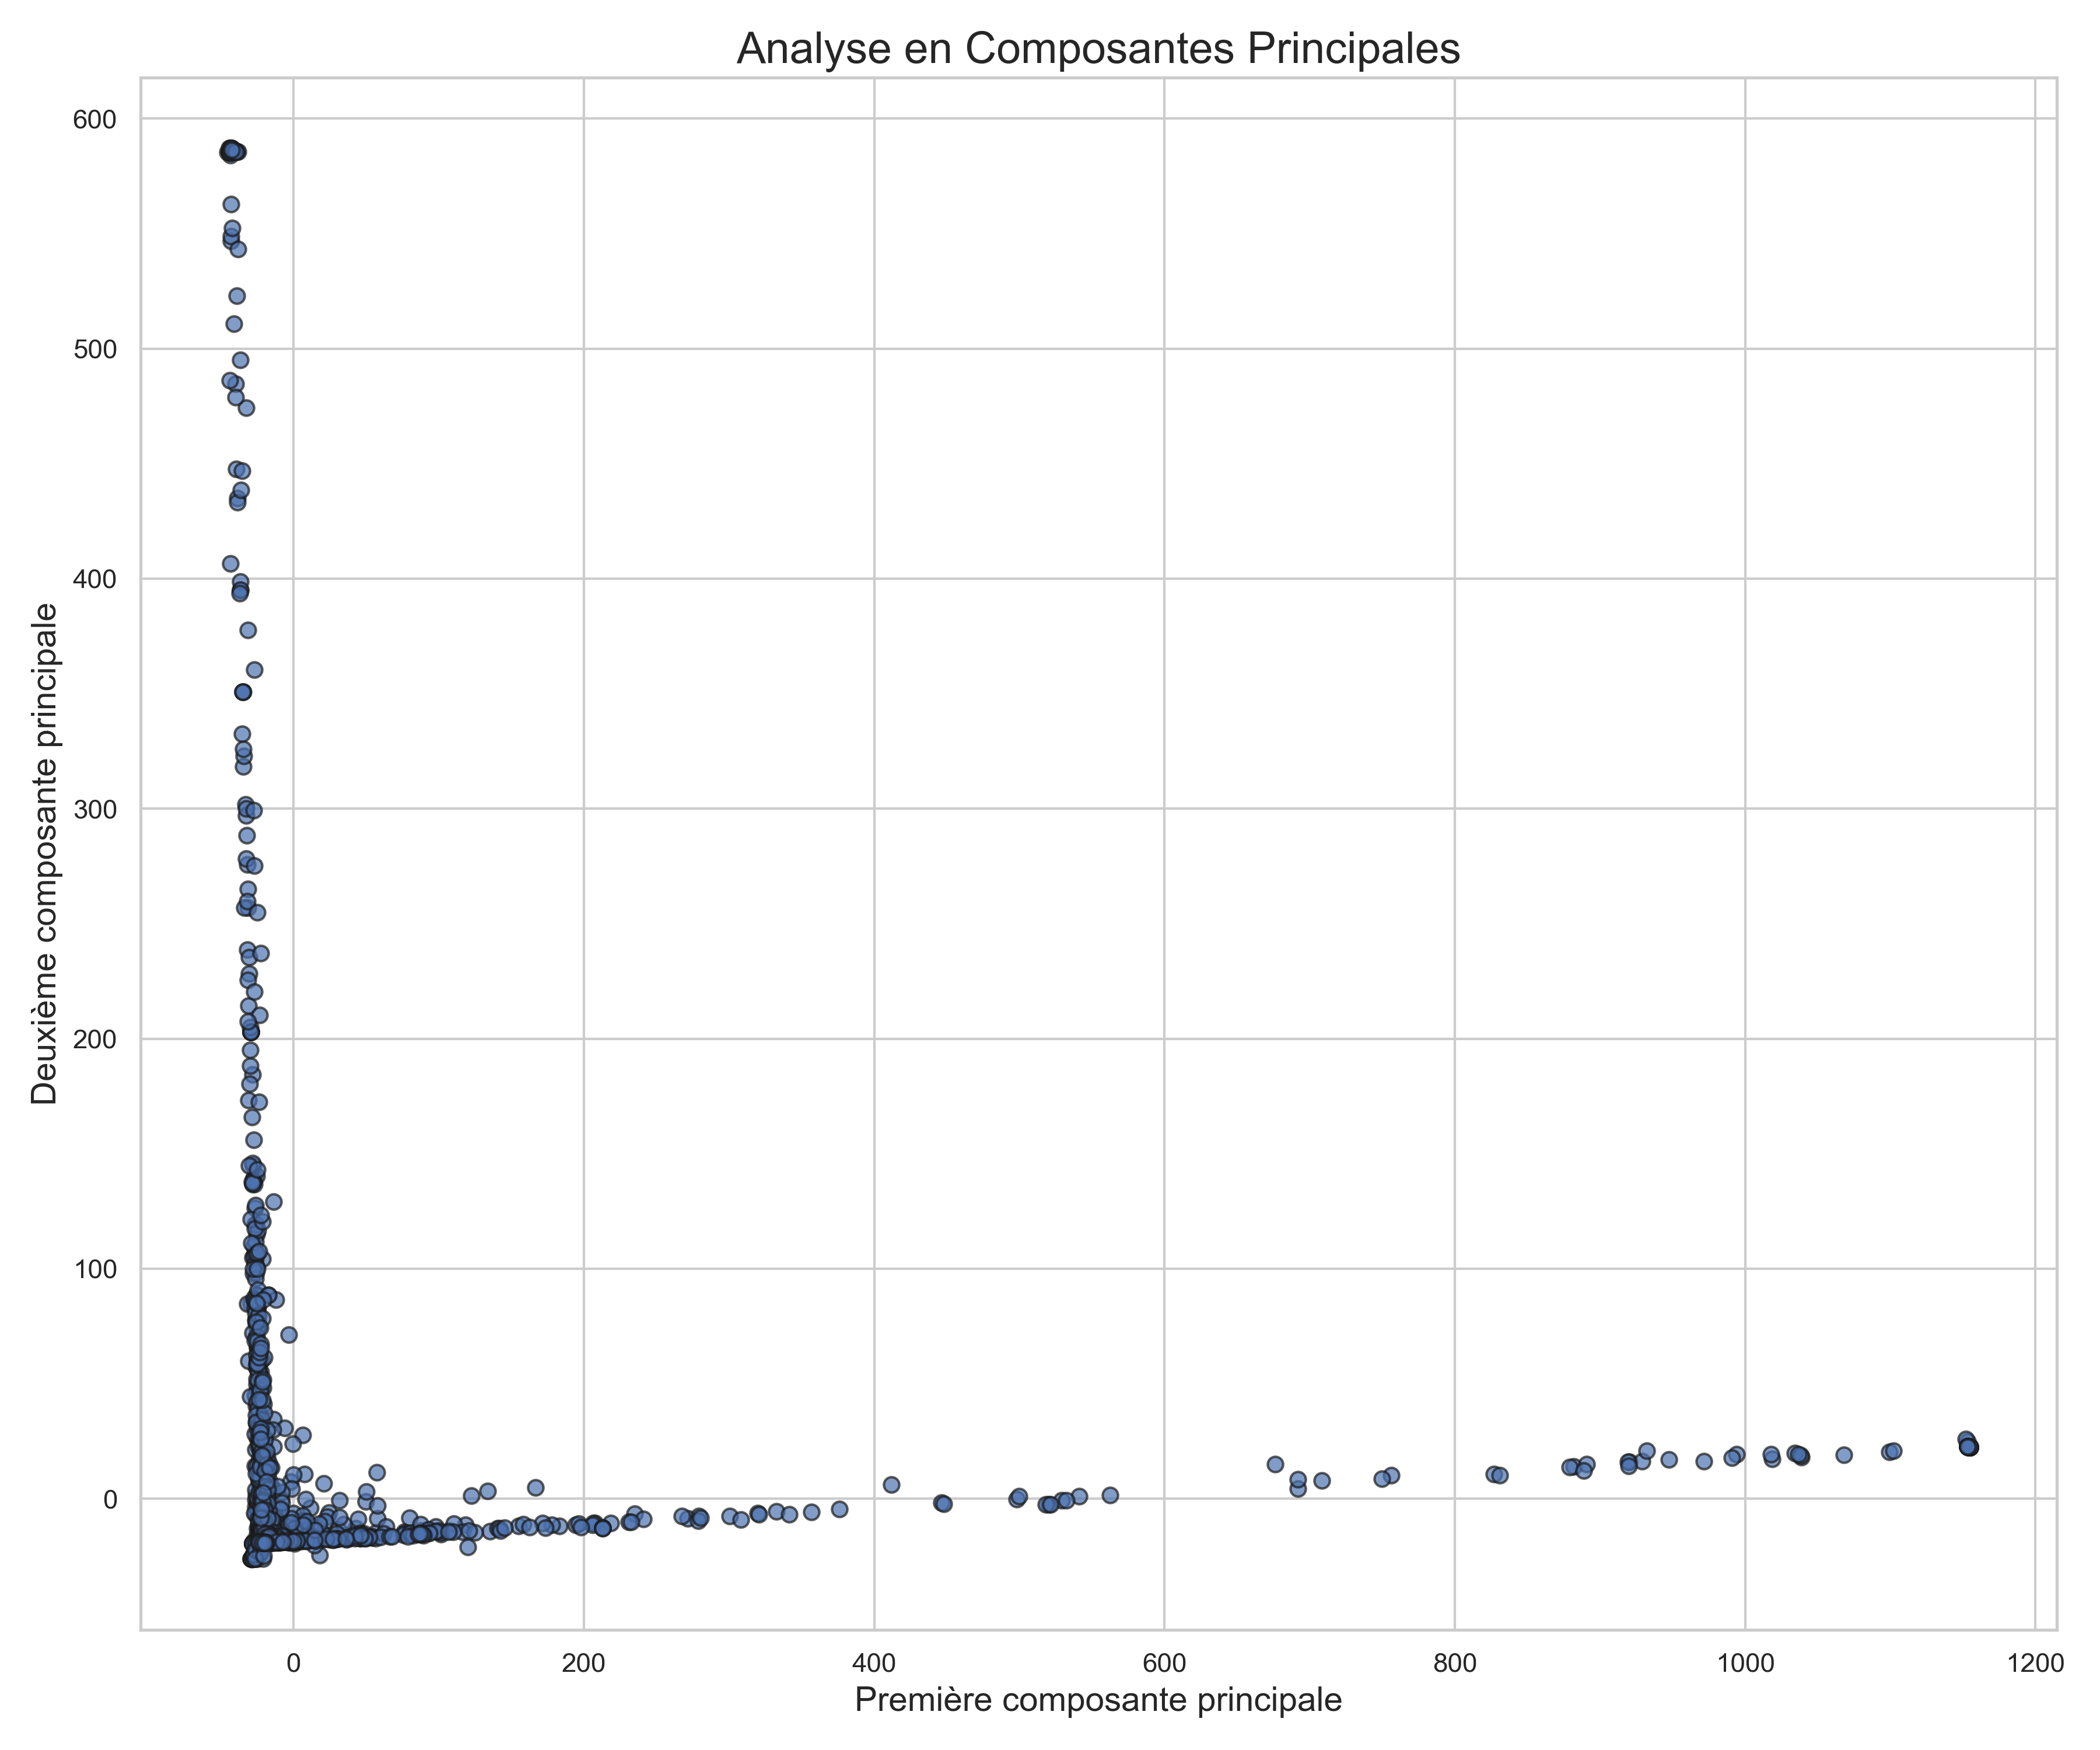
\includegraphics[width=0.8\textwidth]{figures/pca_analysis.png}
    \caption{Projection des entreprises sur les deux premières composantes principales}
    \label{fig:pca_projection}
\end{figure}

\begin{figure}[H]
    \centering
    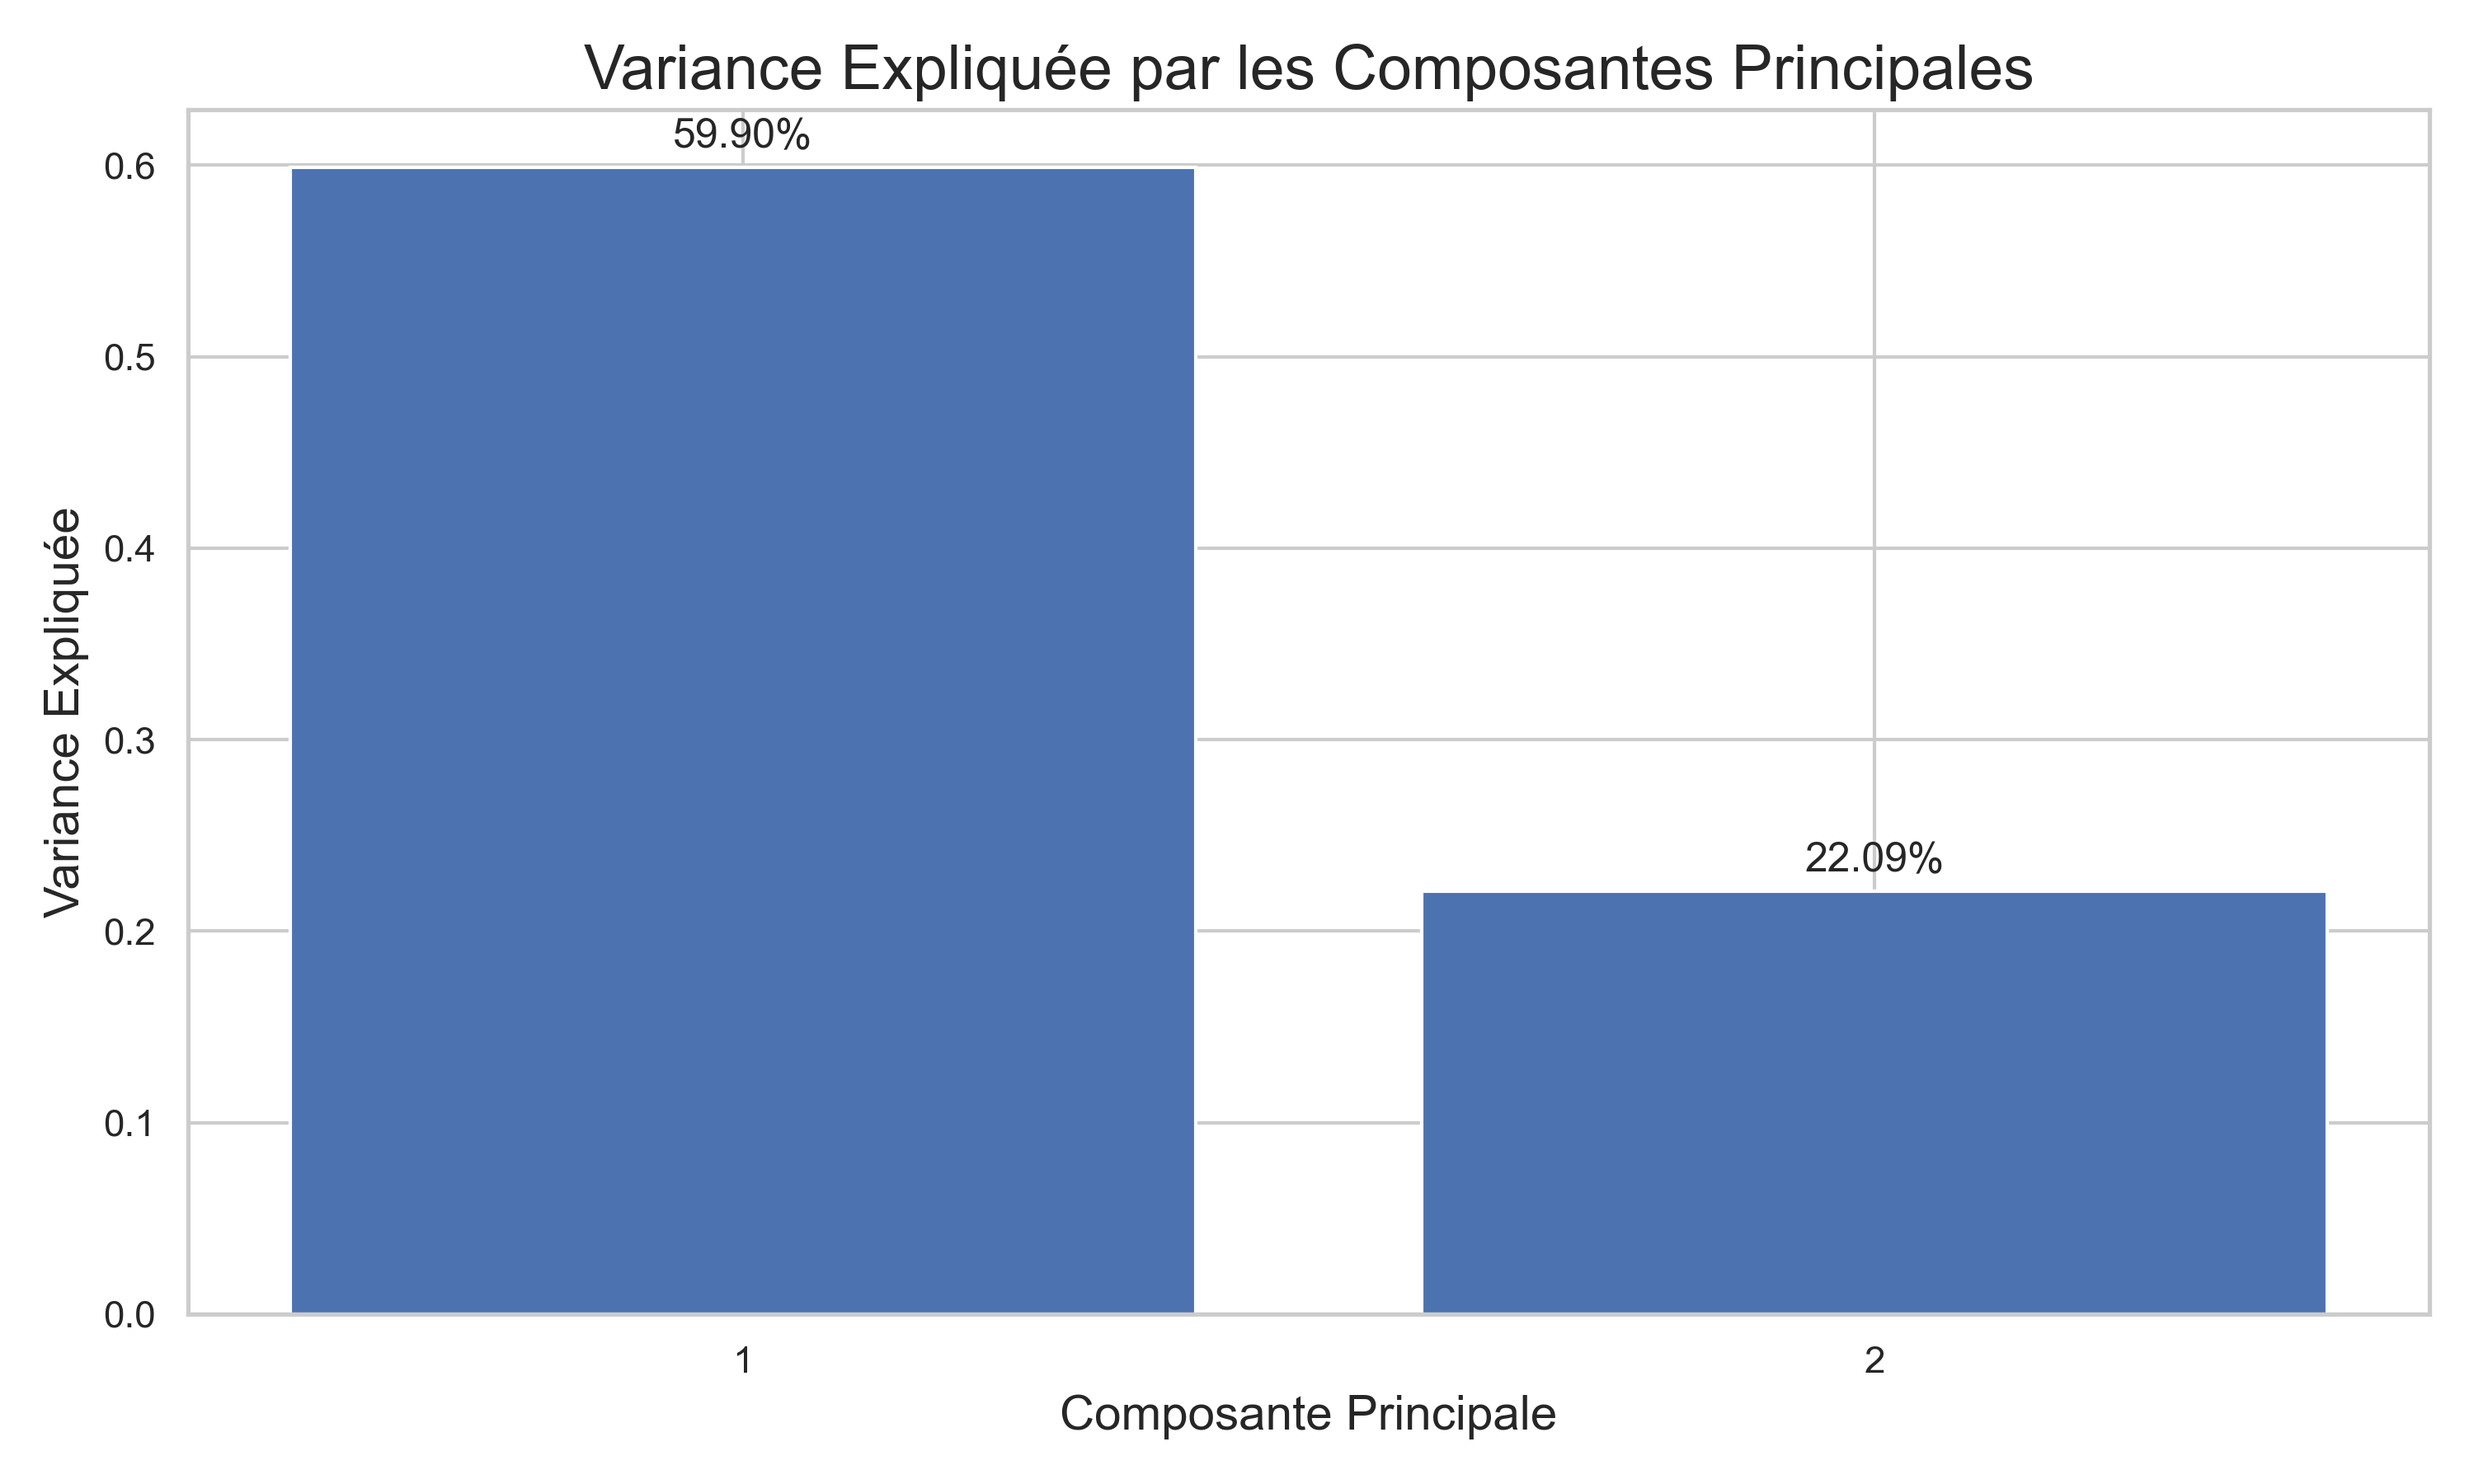
\includegraphics[width=0.8\textwidth]{figures/pca_explained_variance.png}
    \caption{Variance expliquée par les composantes principales}
    \label{fig:pca_variance}
\end{figure}

\begin{figure}[H]
    \centering
    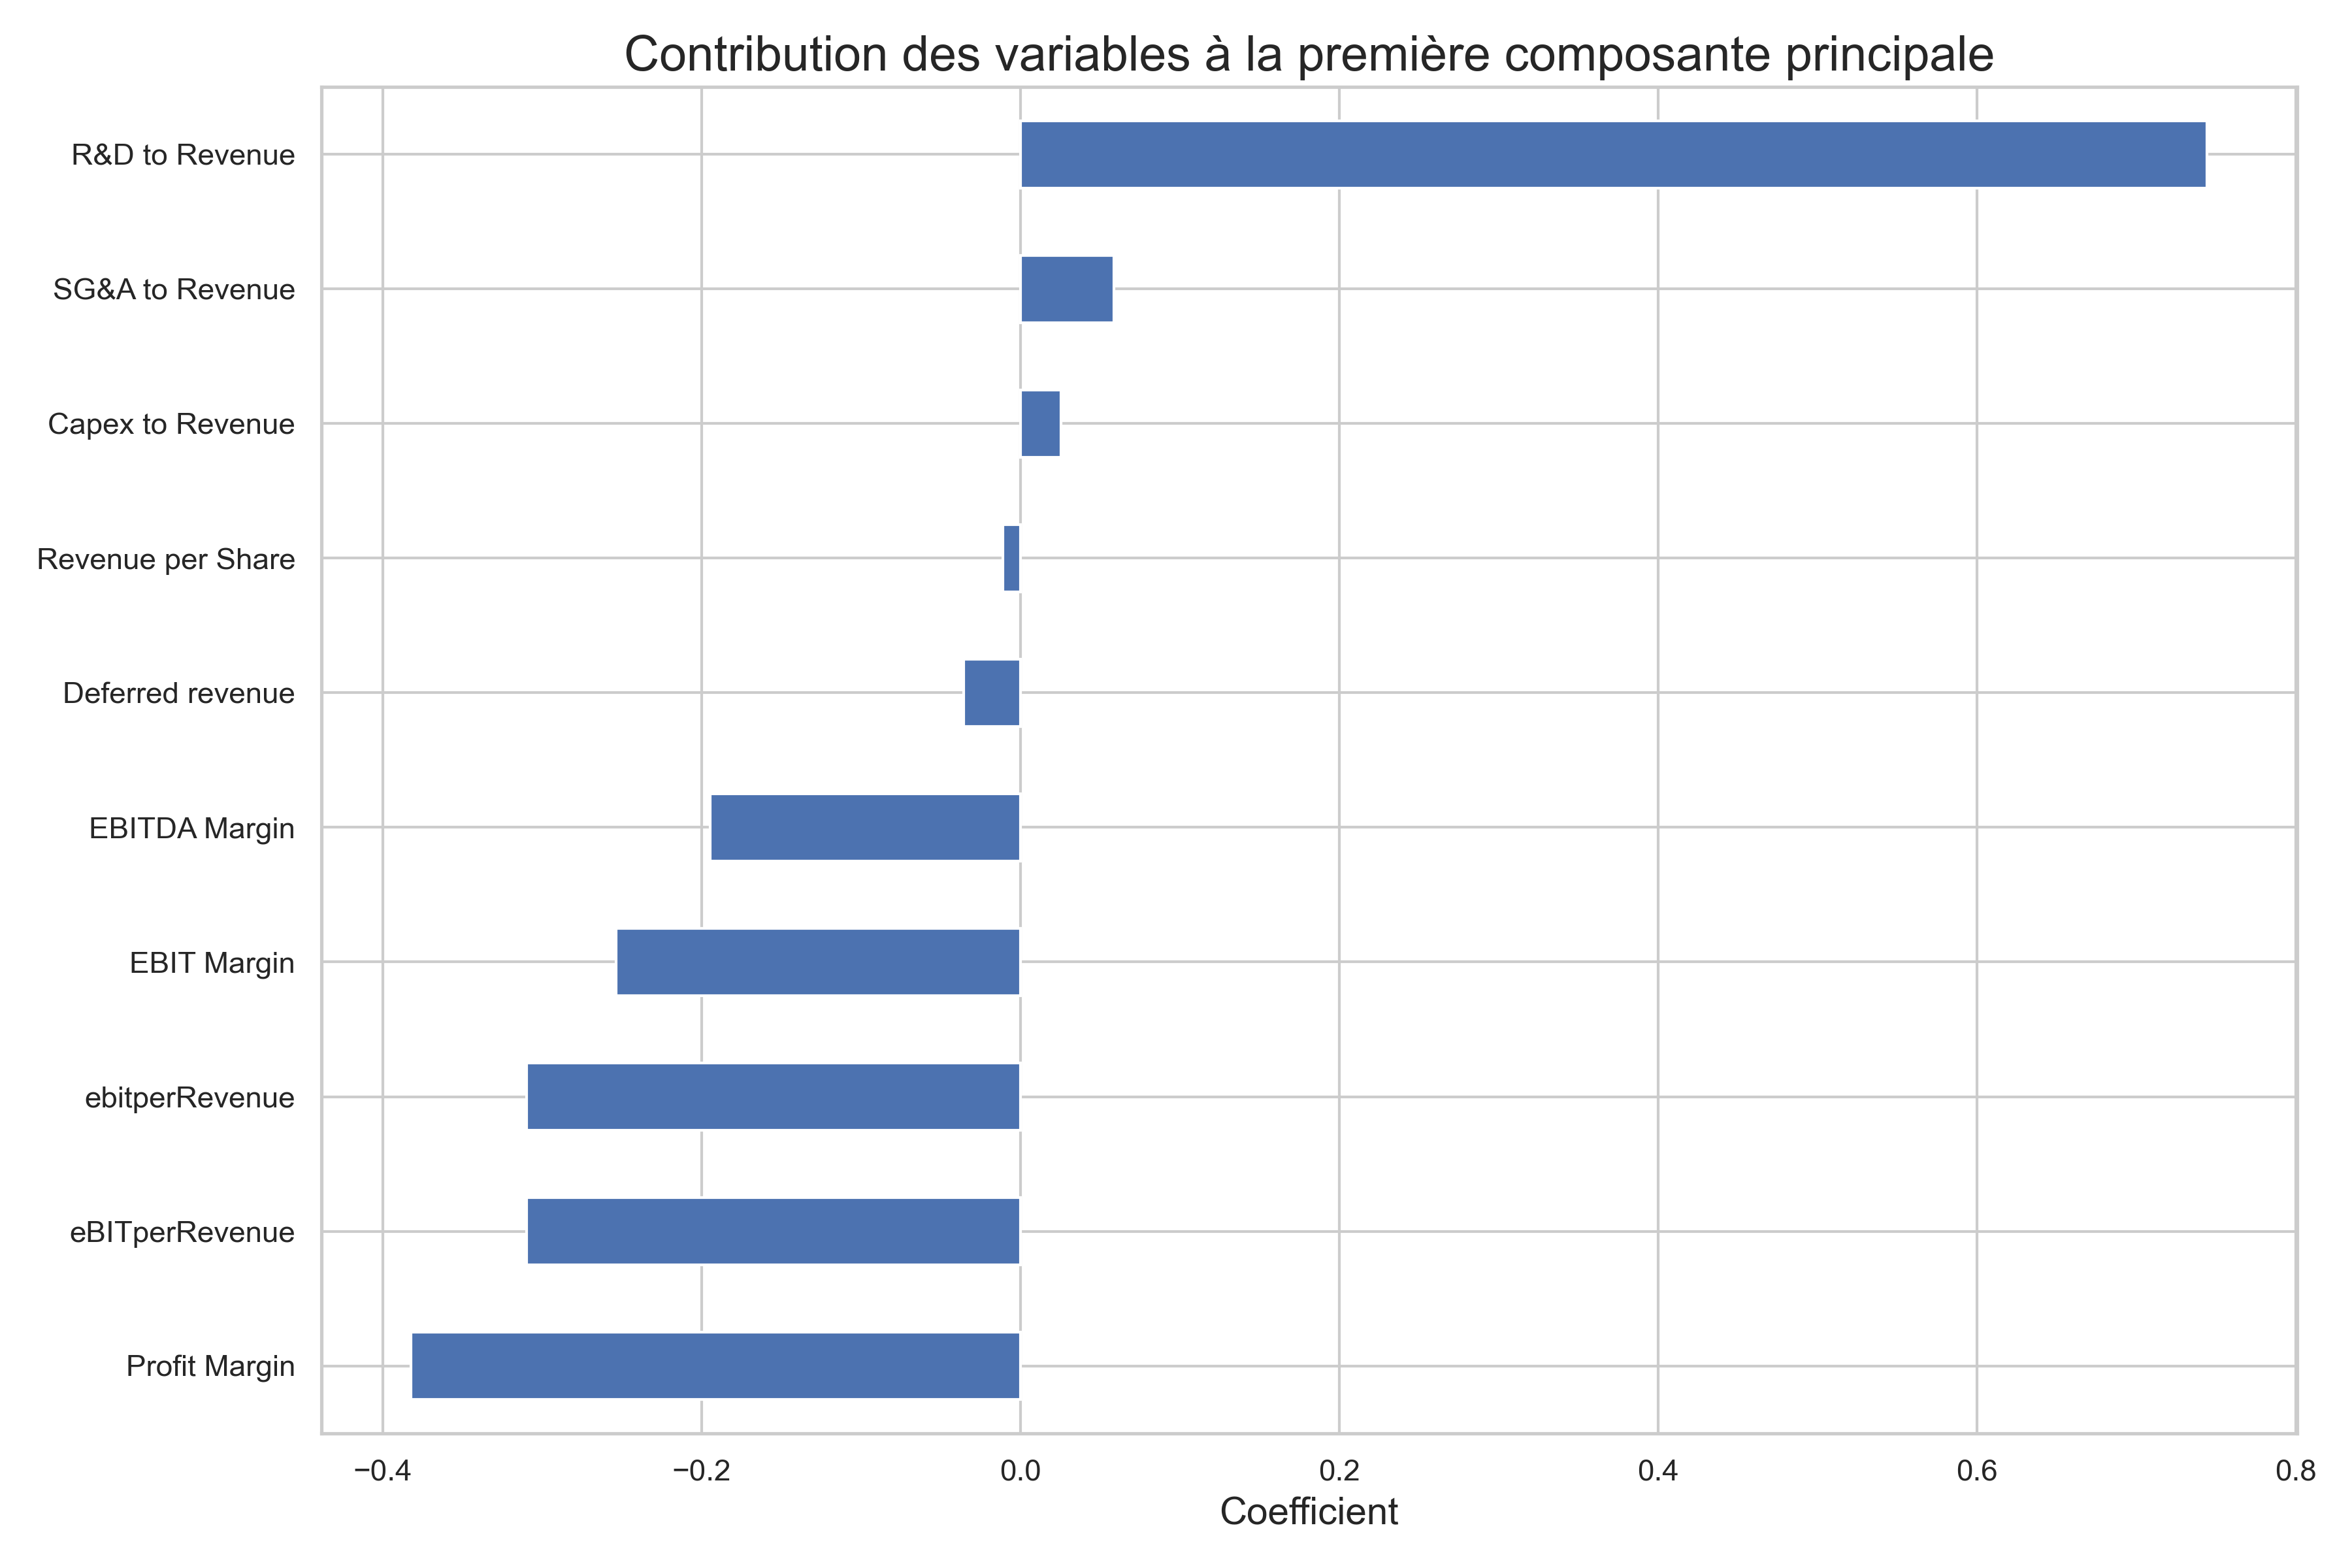
\includegraphics[width=0.8\textwidth]{figures/pca_loadings_pc1.png}
    \caption{Contribution des variables à la première composante principale}
    \label{fig:pca_loadings}
\end{figure}

La figure \ref{fig:pca_projection} montre la projection des entreprises sur les deux premières composantes principales, qui captent la plus grande partie de la variance dans les données. La figure \ref{fig:pca_variance} illustre la proportion de variance expliquée par chaque composante principale. La figure \ref{fig:pca_loadings} présente les variables qui contribuent le plus à la première composante principale, révélant ainsi les facteurs financiers les plus discriminants dans notre jeu de données. Cette analyse nous permet de réduire la complexité des données tout en conservant l'information essentielle, facilitant ainsi la visualisation et l'interprétation des patterns dans les données financières.

\section{Classification des entreprises par K-Means}
L'algorithme K-Means nous a permis de regrouper les entreprises en clusters selon leurs profils financiers. Cette approche non supervisée révèle des groupes naturels d'entreprises ayant des caractéristiques similaires.

\begin{figure}[H]
    \centering
    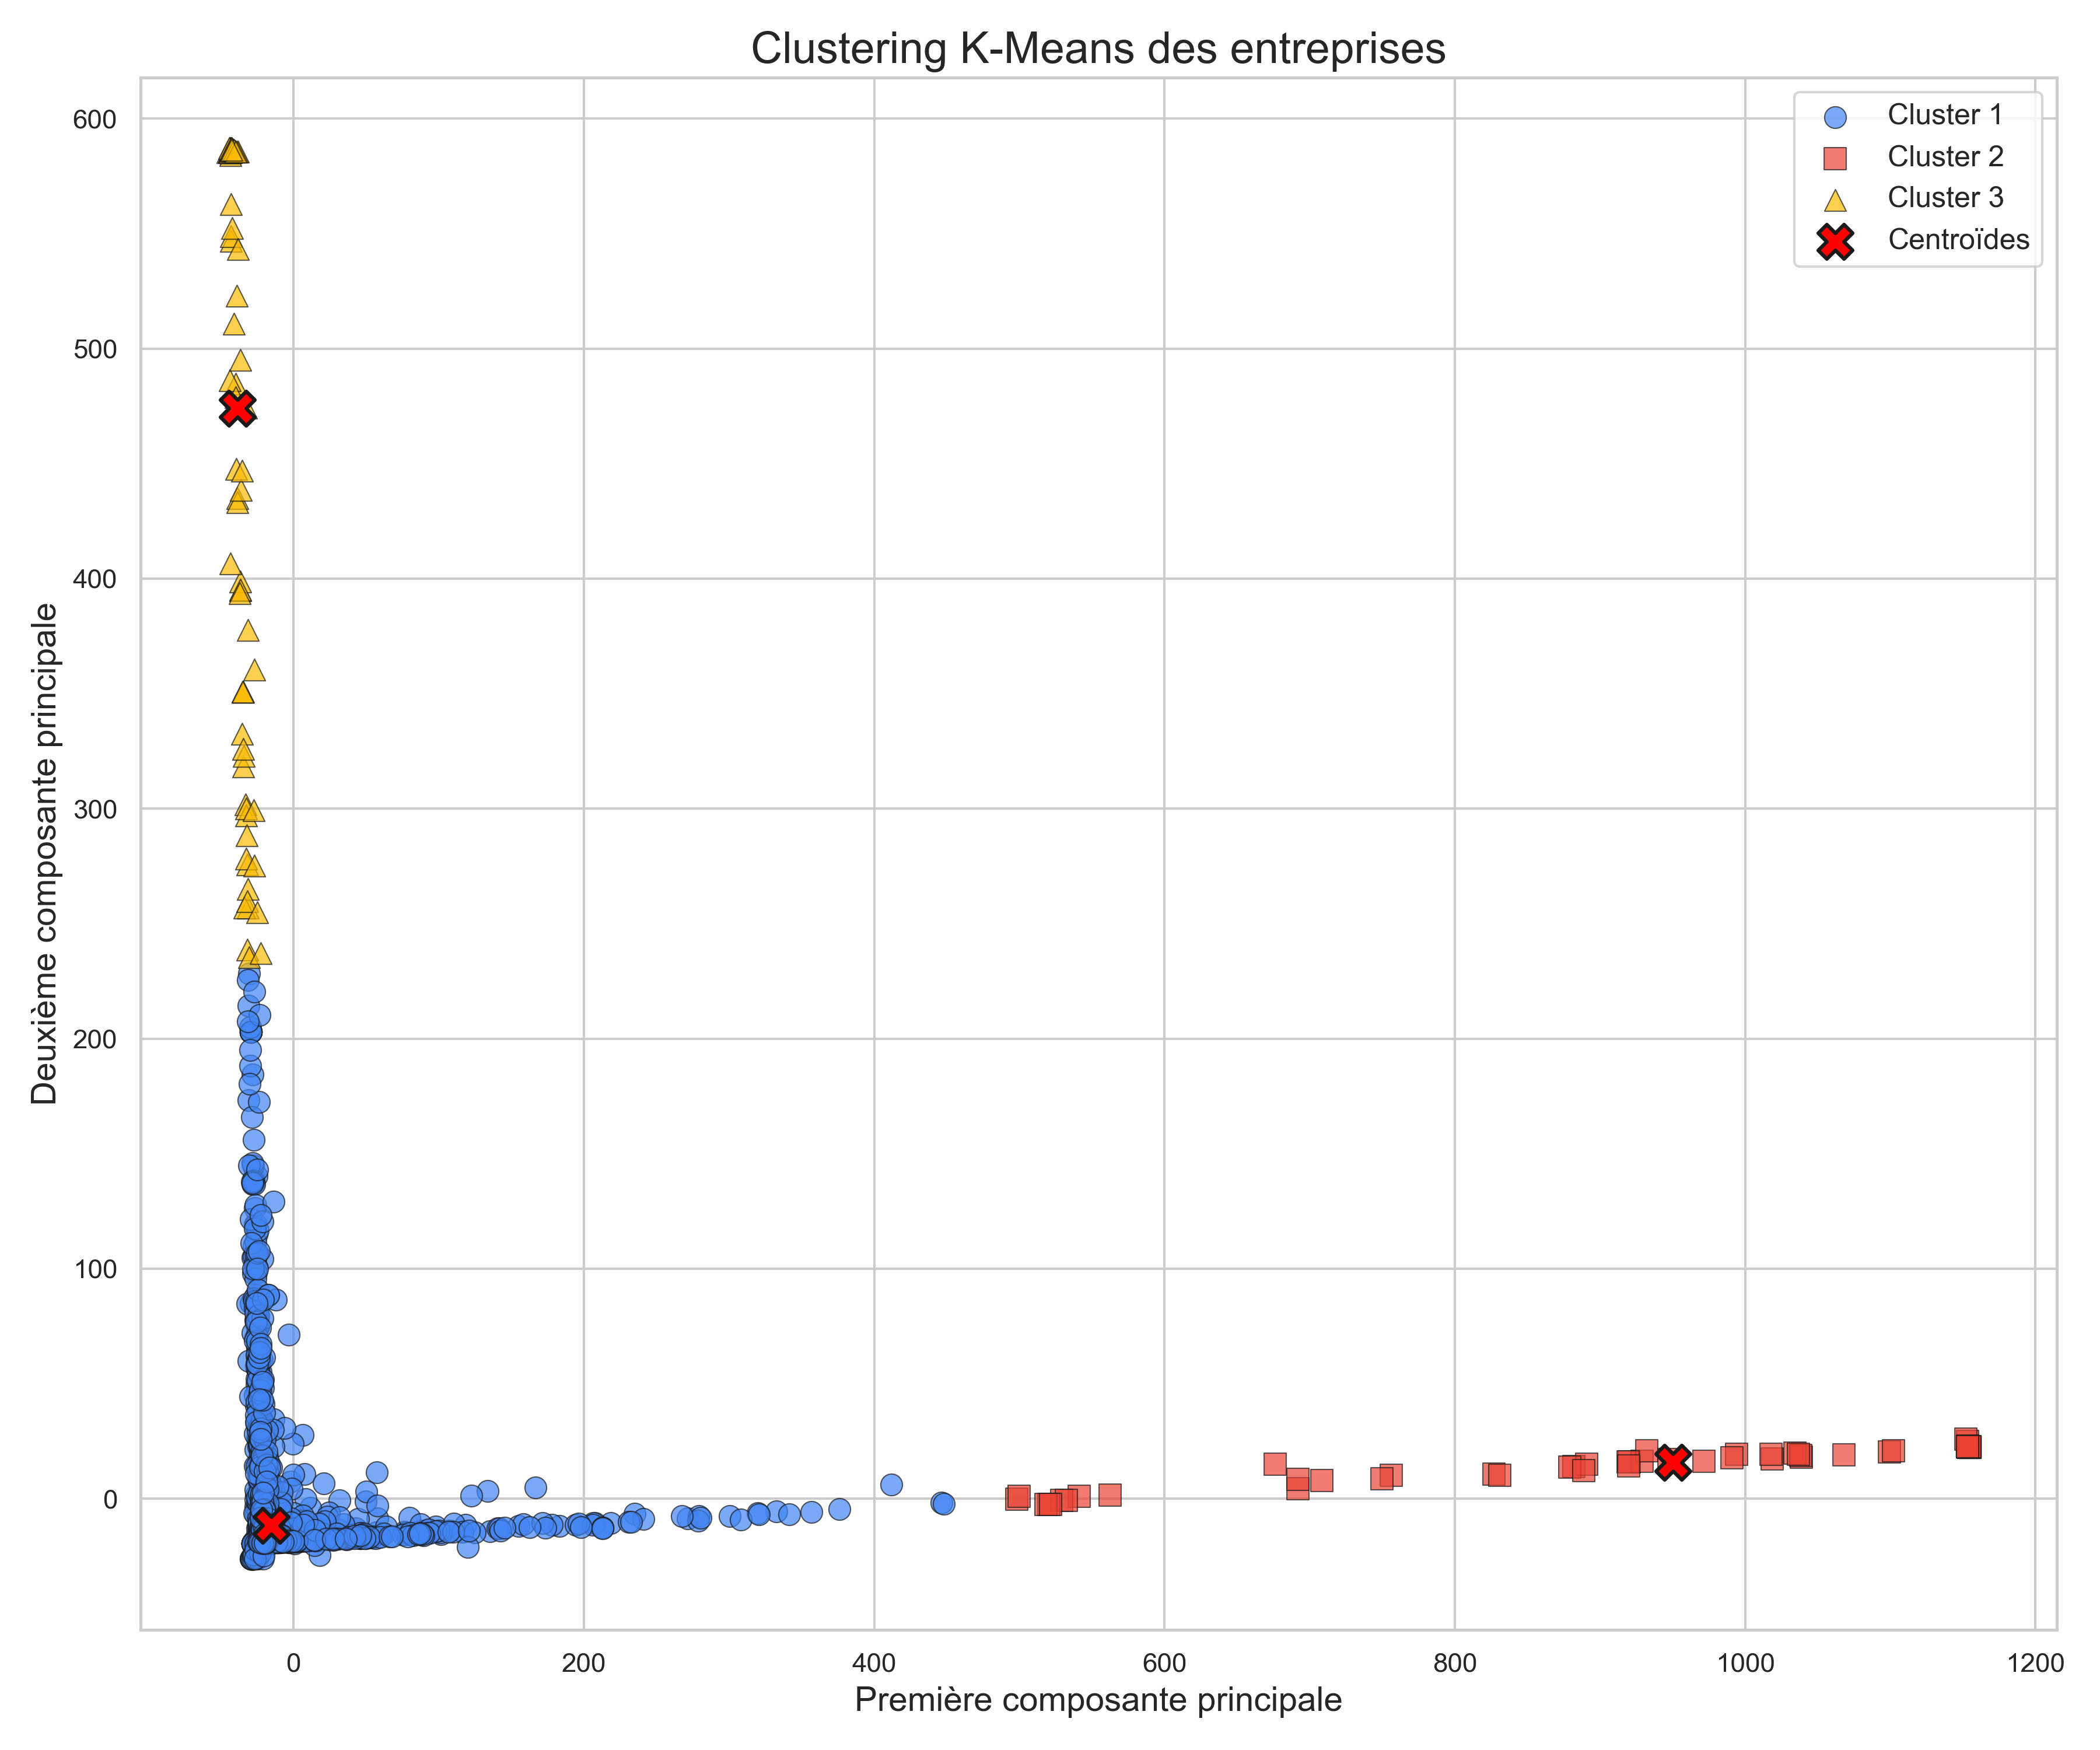
\includegraphics[width=0.85\textwidth]{figures/kmeans_clusters.png}
    \caption{Clusters d'entreprises identifiés par l'algorithme K-Means}
    \label{fig:kmeans_clusters}
\end{figure}

\section{Interprétation des clusters}
Une fois les clusters identifiés, nous avons analysé leurs caractéristiques pour comprendre ce qui distingue chaque groupe et proposer une interprétation financière et économique.

\begin{figure}[H]
    \centering
    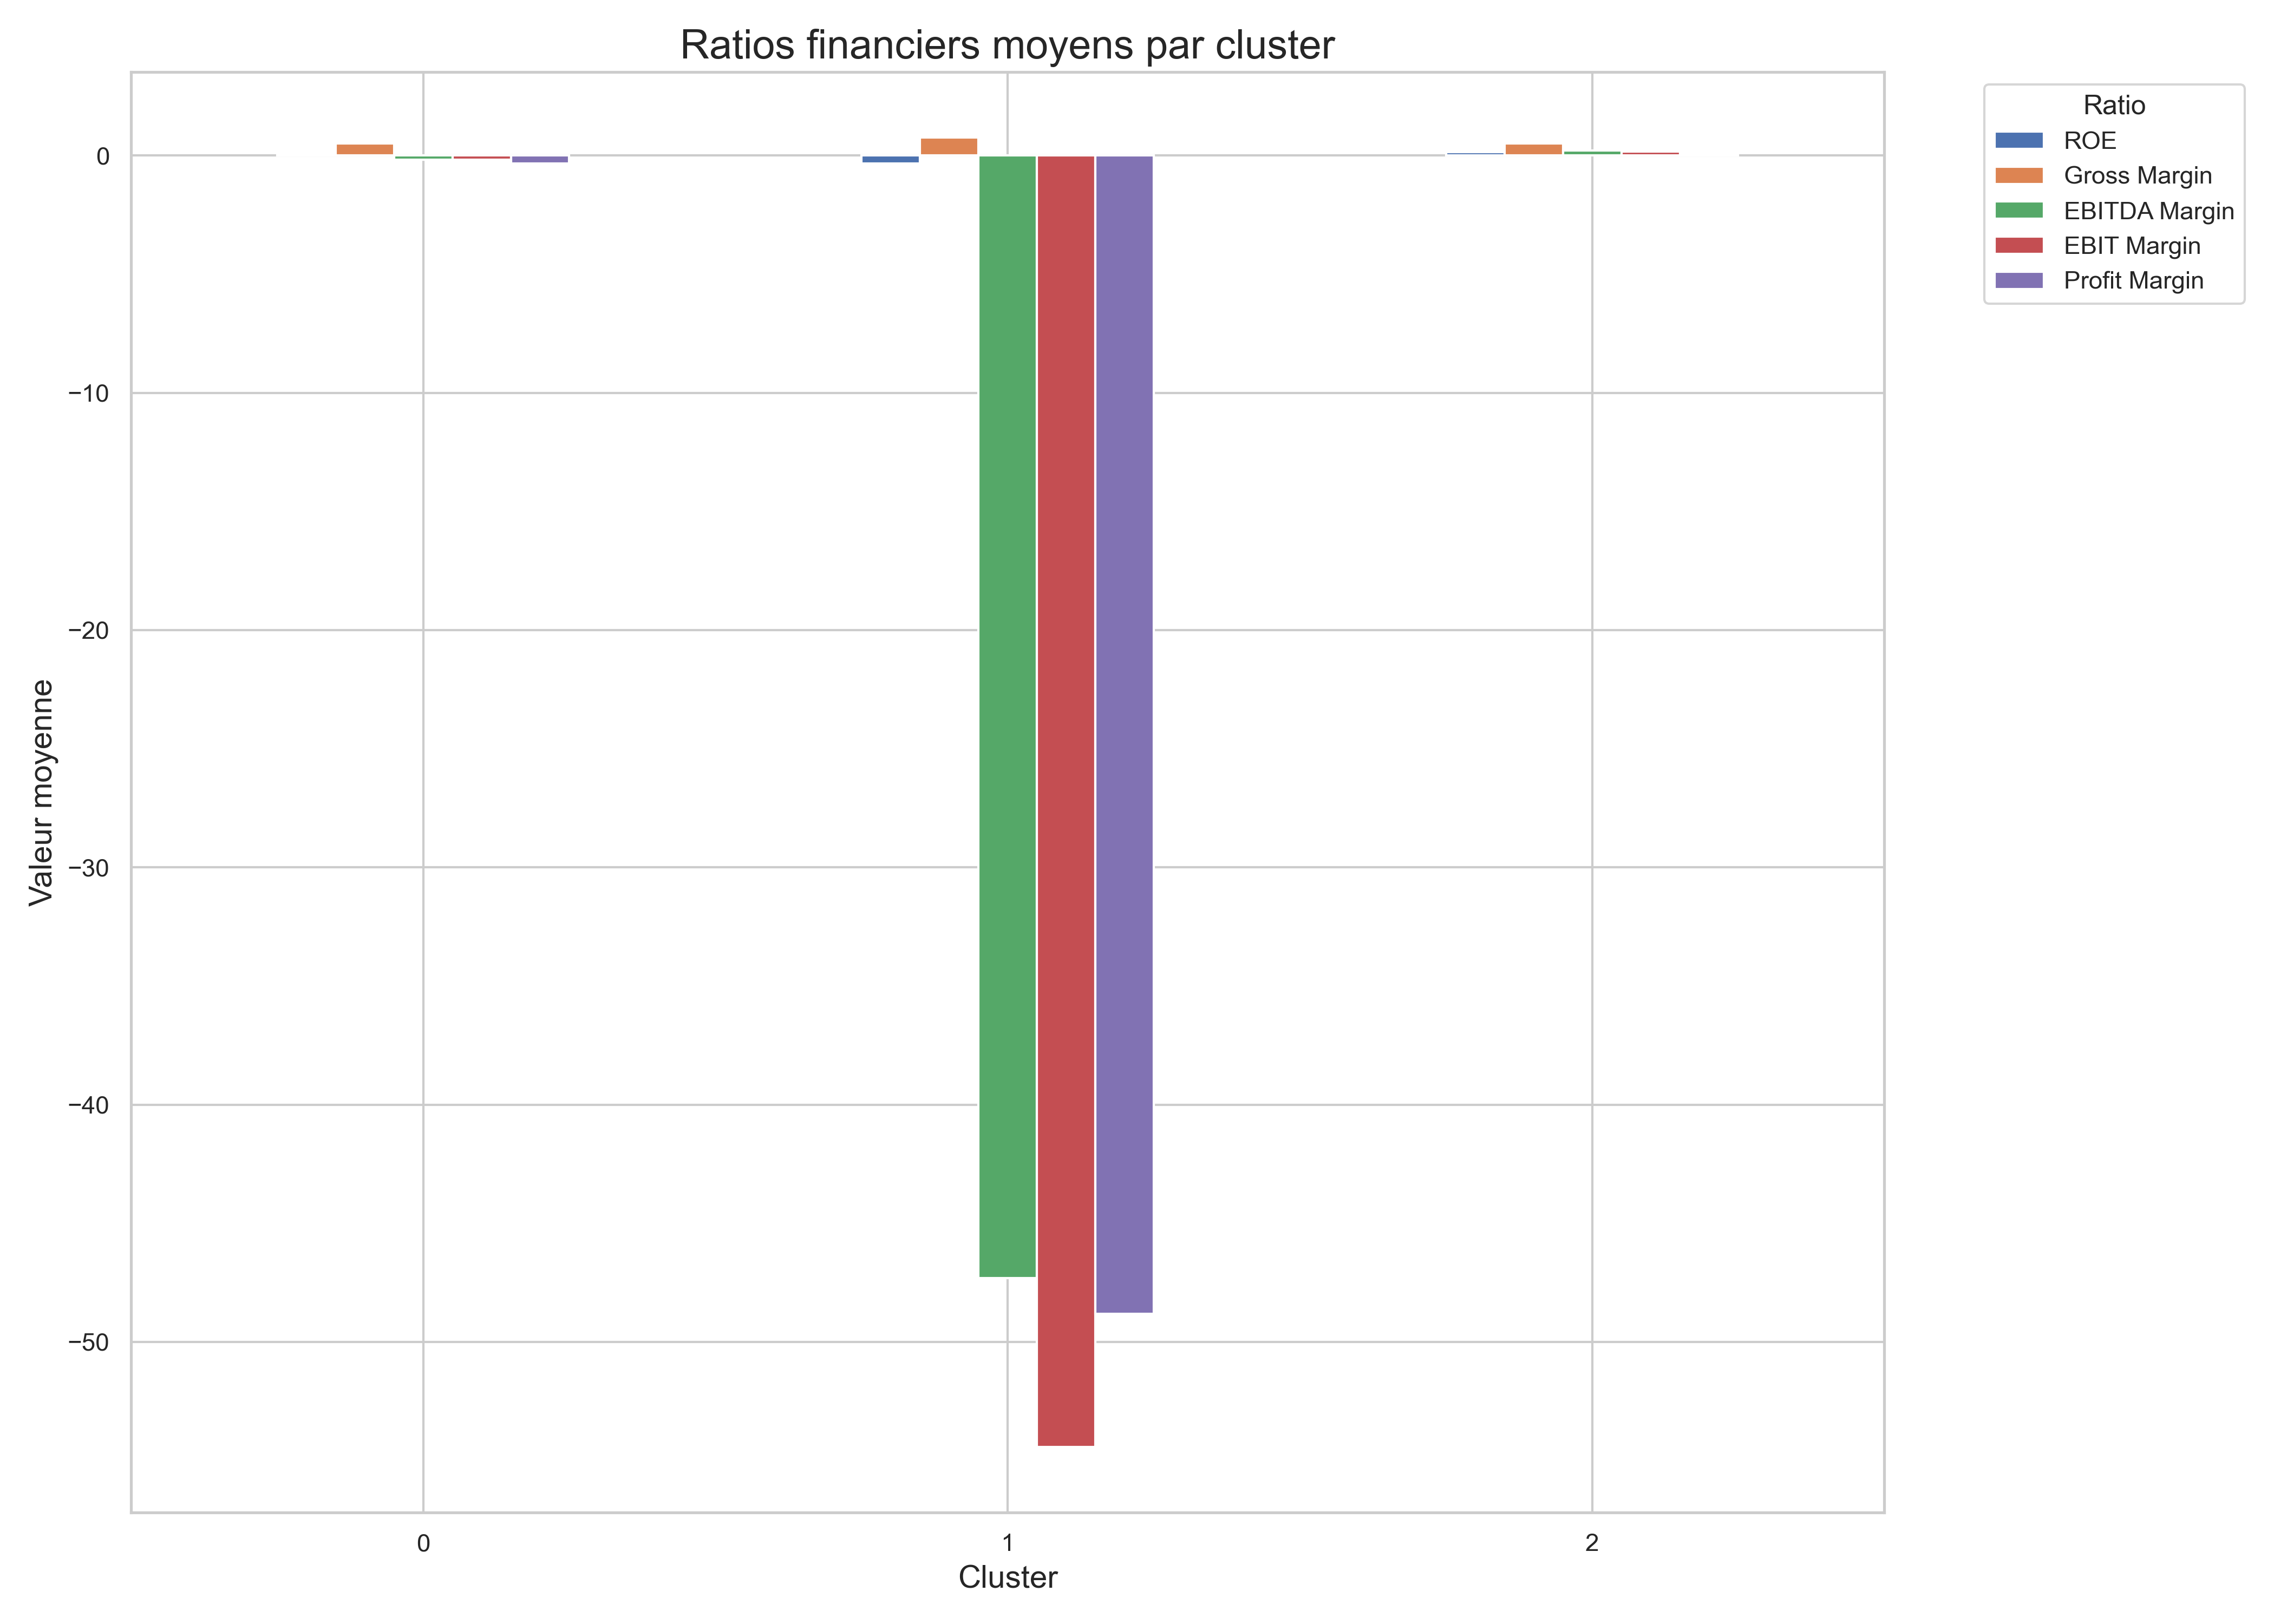
\includegraphics[width=0.95\textwidth]{figures/financial_ratios_by_cluster.png}
    \caption{Ratios financiers moyens par cluster}
    \label{fig:ratios_by_cluster}
\end{figure}

\begin{figure}[H]
    \centering
    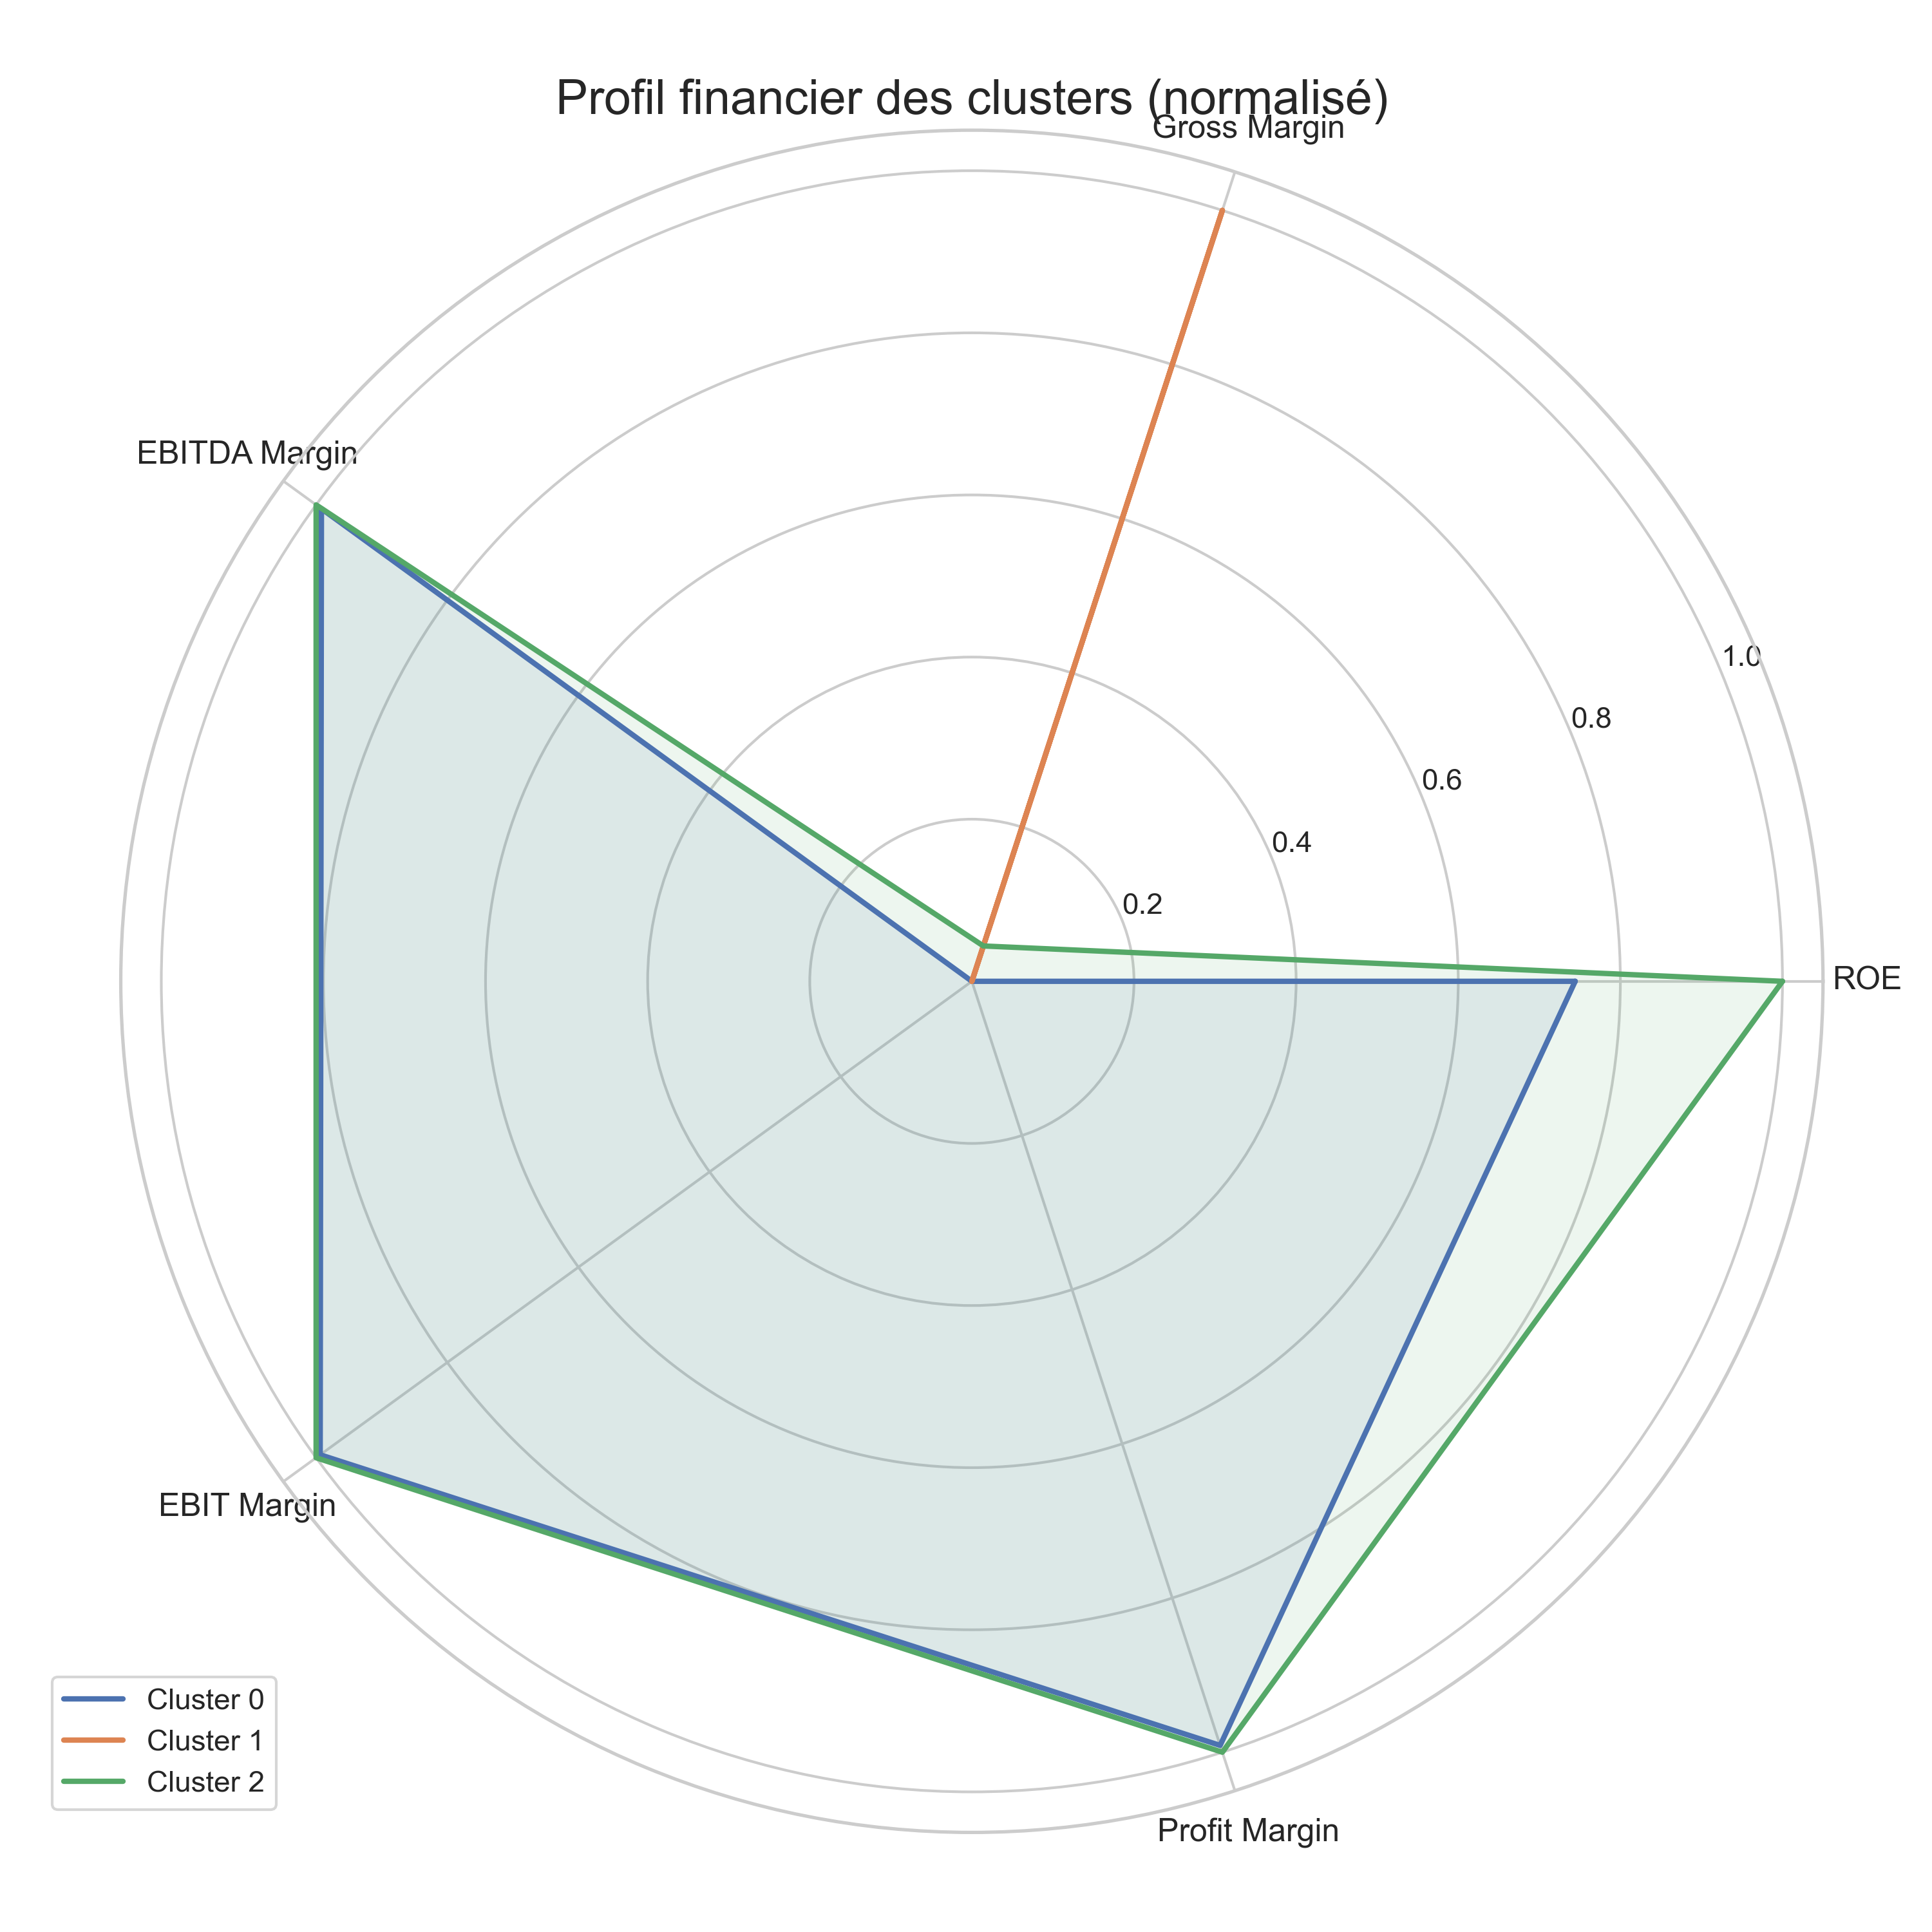
\includegraphics[width=0.95\textwidth]{figures/cluster_radar_chart.png}
    \caption{Profil financier des clusters (normalisé)}
    \label{fig:cluster_radar}
\end{figure}

\begin{figure}[H]
    \centering
    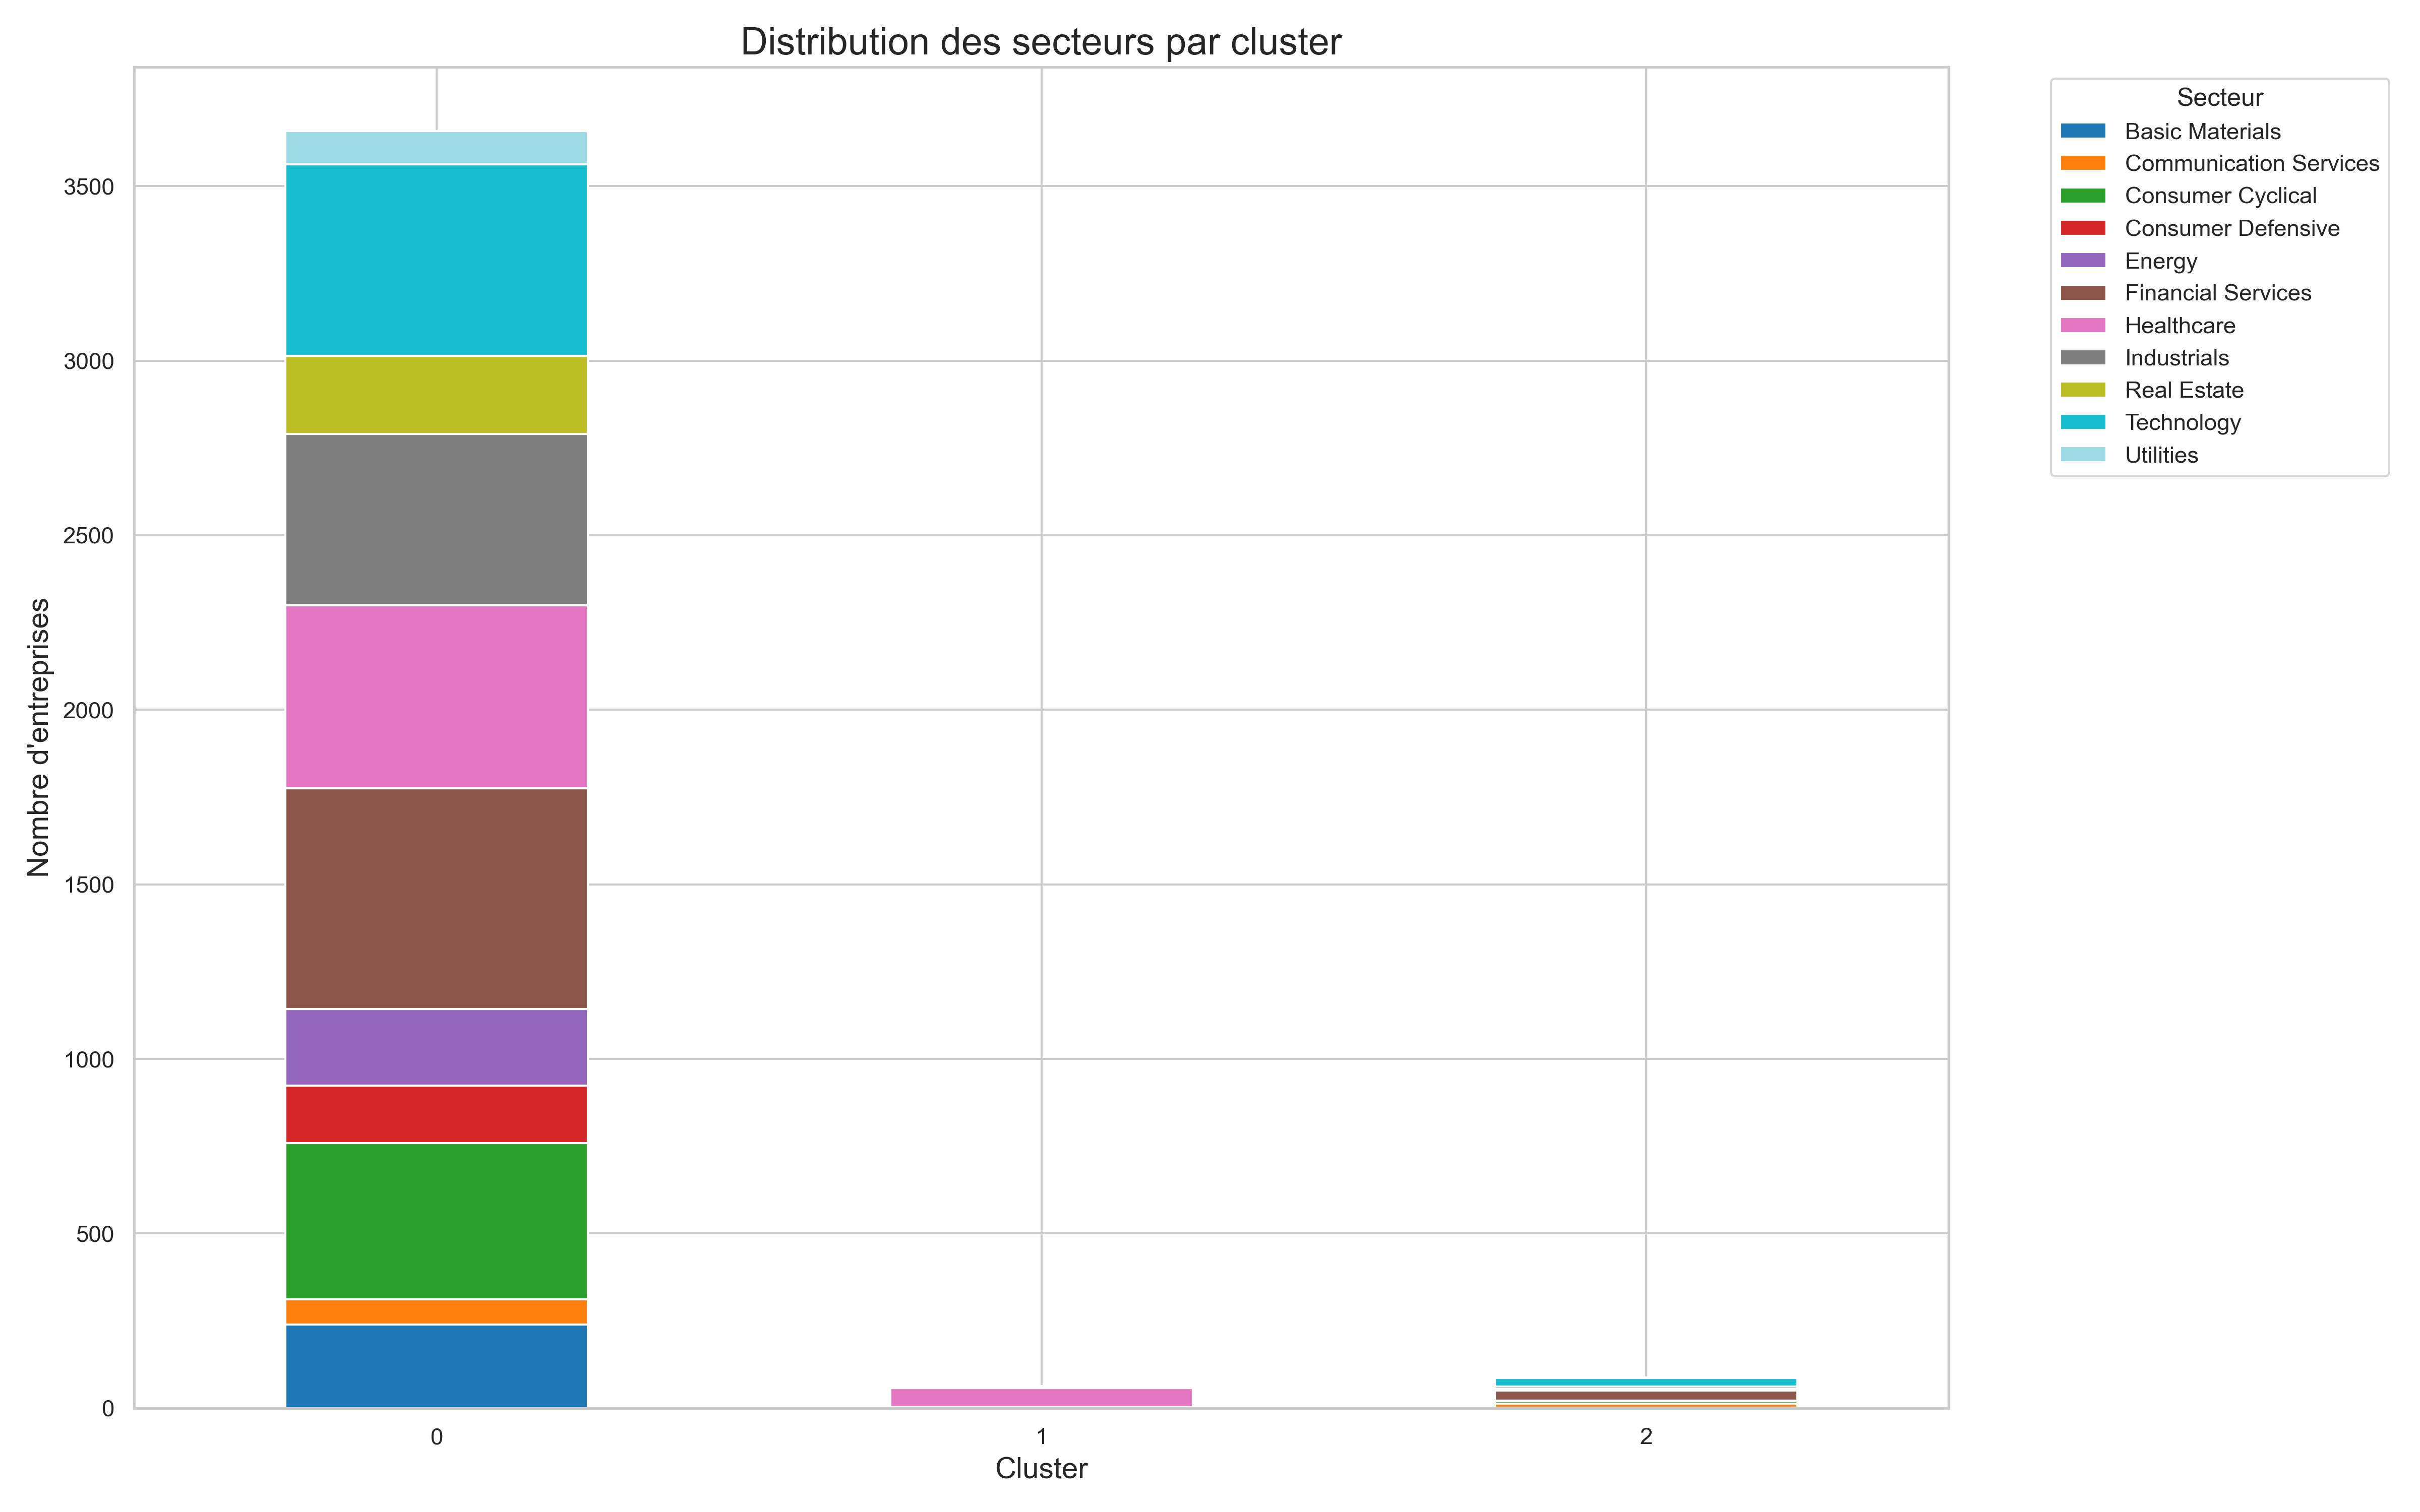
\includegraphics[width=0.95\textwidth]{figures/sector_distribution_by_cluster.png}
    \caption{Distribution des secteurs par cluster}
    \label{fig:sector_by_cluster}
\end{figure}

\begin{figure}[H]
    \centering
    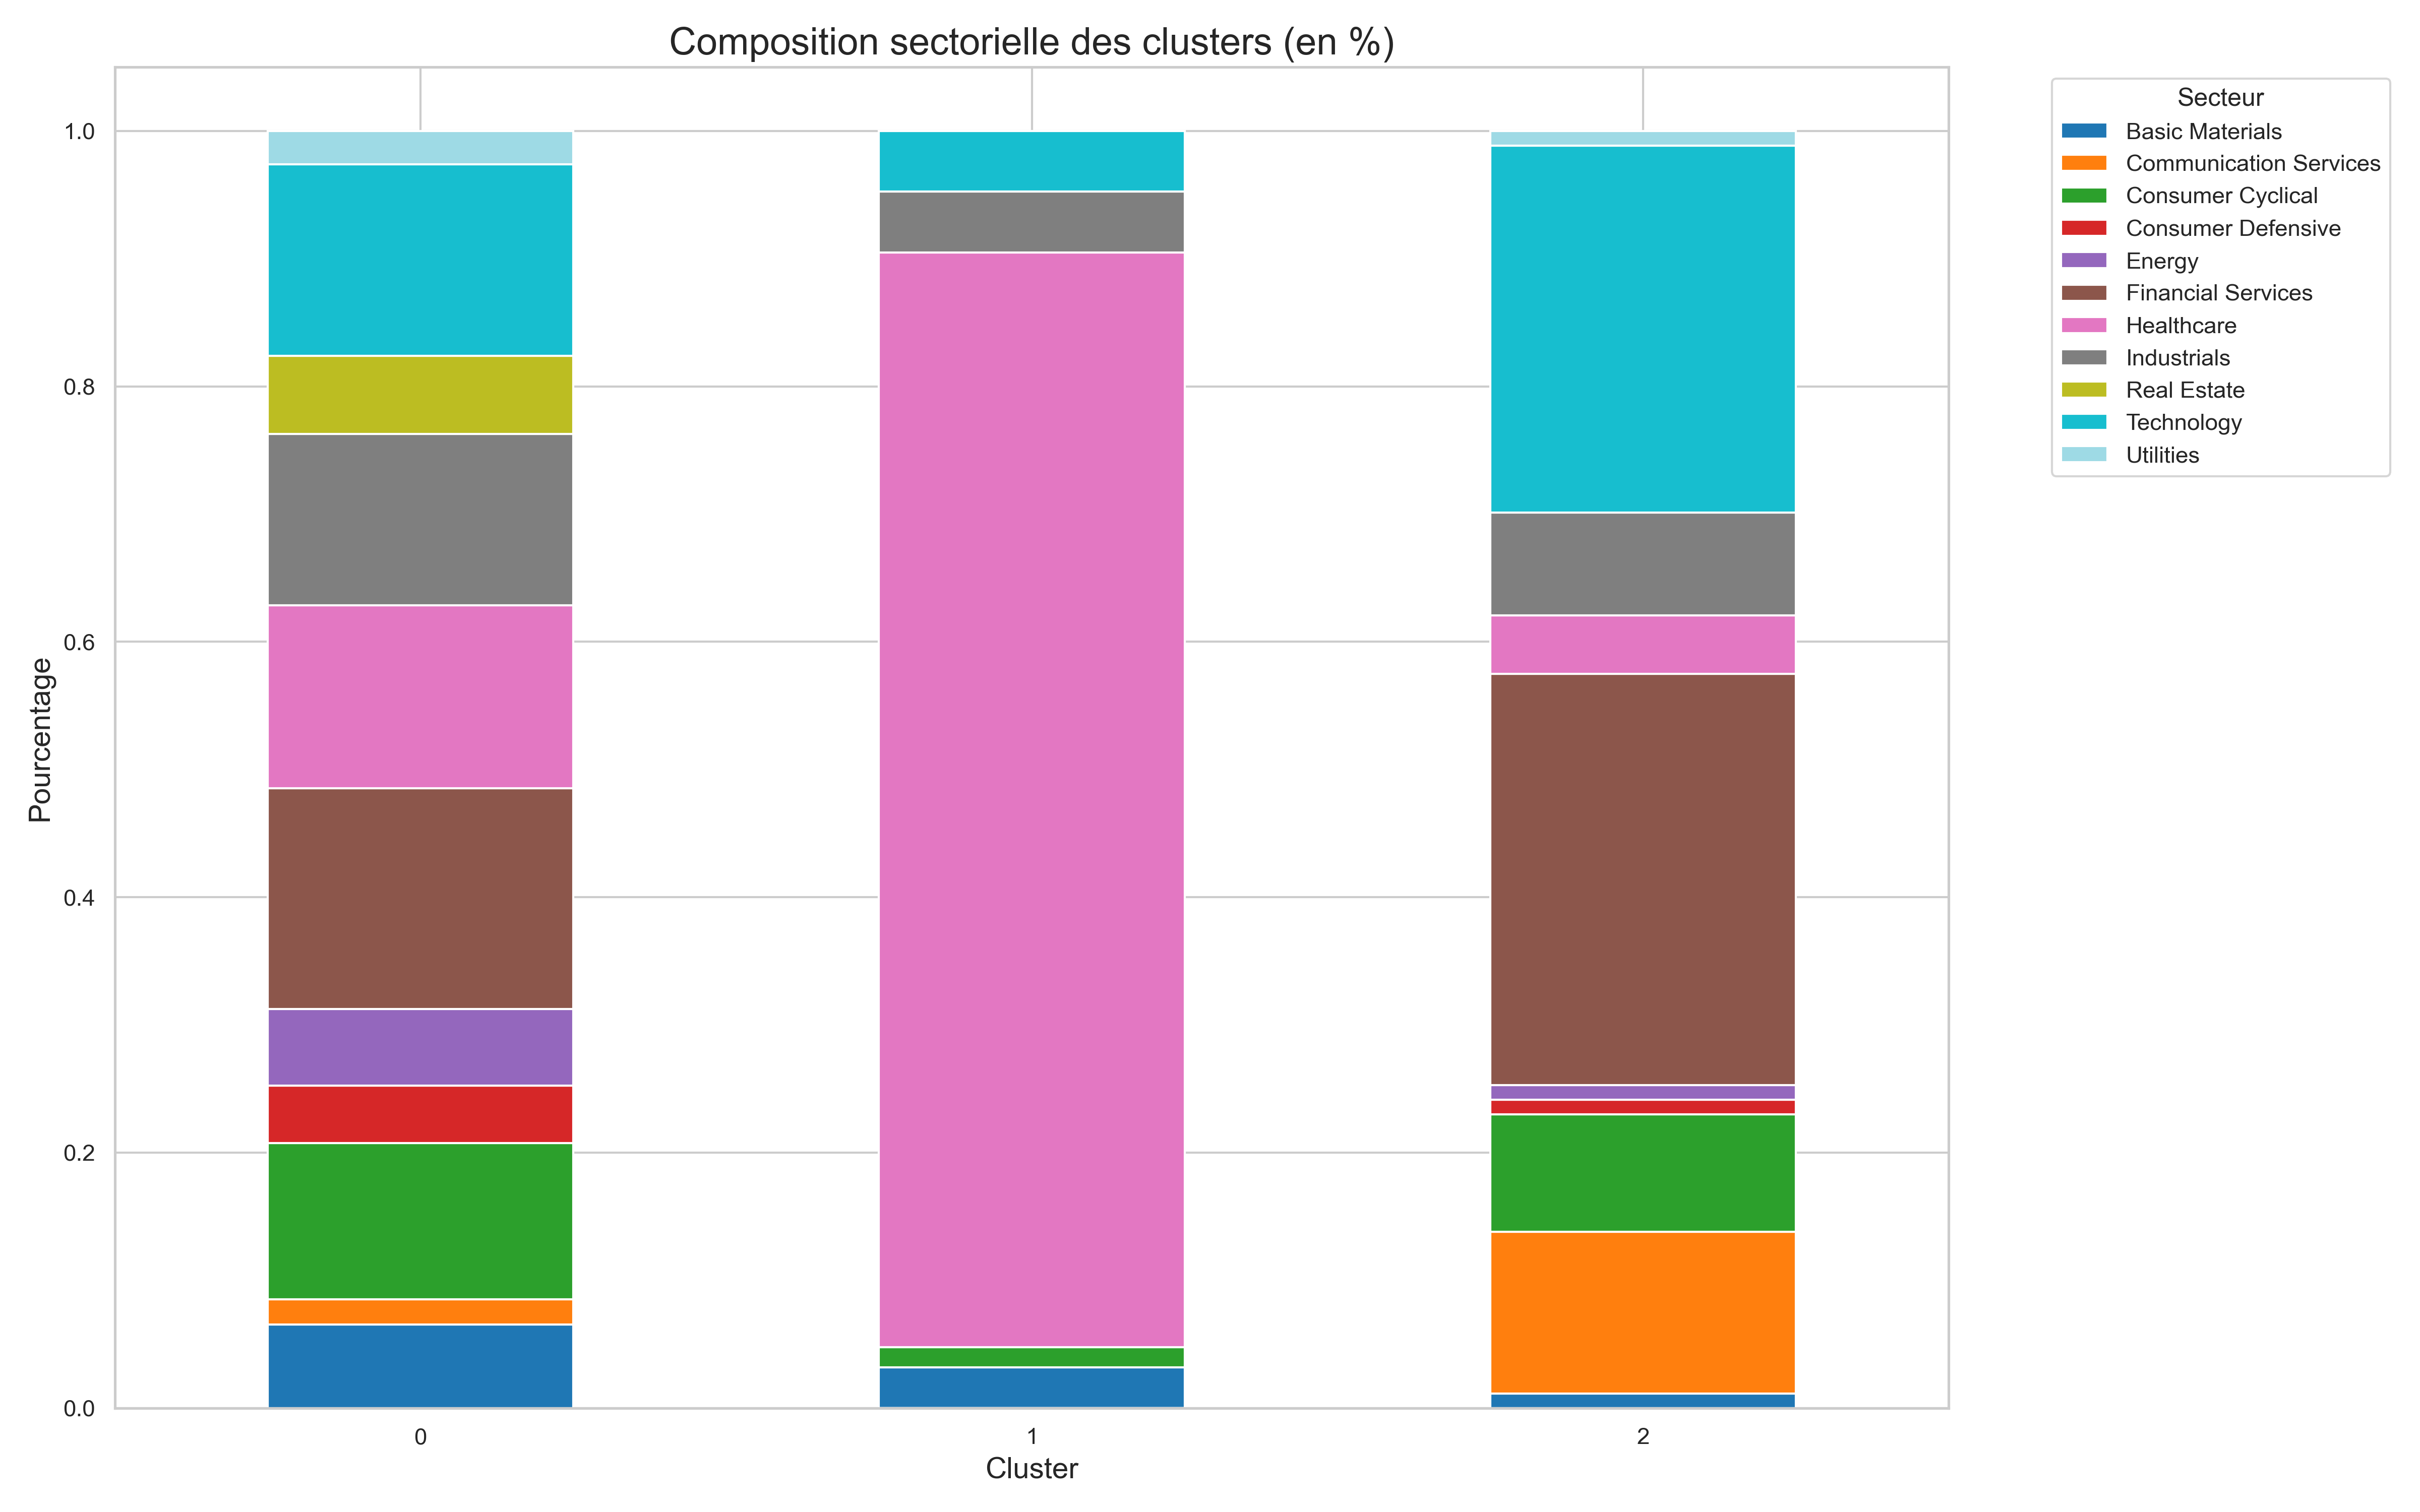
\includegraphics[width=0.95\textwidth]{figures/sector_percentage_by_cluster.png}
    \caption{Composition sectorielle des clusters (en \%)}
    \label{fig:sector_percentage}
\end{figure}

Les figures \ref{fig:kmeans_clusters}, \ref{fig:ratios_by_cluster}, \ref{fig:cluster_radar}, \ref{fig:sector_by_cluster} et \ref{fig:sector_percentage} présentent les résultats de notre analyse de clustering. La figure \ref{fig:kmeans_clusters} montre la répartition des entreprises dans l'espace réduit de l'ACP, avec les trois clusters identifiés clairement visibles. La figure \ref{fig:ratios_by_cluster} compare les ratios financiers moyens entre les clusters, tandis que la figure \ref{fig:cluster_radar} offre une visualisation radar permettant de comparer facilement les profils financiers des différents clusters. Enfin, les figures \ref{fig:sector_by_cluster} et \ref{fig:sector_percentage} illustrent la composition sectorielle de chaque cluster, révélant des affinités intéressantes entre certains secteurs d'activité et les profils financiers identifiés.

\chapter{Modélisation prédictive}
\section{Modèles d'arbres de décision et Random Forest}
Les modèles basés sur les arbres de décision, notamment les Random Forests, sont particulièrement bien adaptés pour identifier les facteurs clés influençant les variables cibles financières. Nous avons construit et évalué ces modèles sur notre jeu de données.

Pour notre modélisation prédictive, nous avons implémenté des modèles d'arbres de décision et de Random Forest, qui sont particulièrement adaptés aux données financières en raison de leur capacité à capturer des relations non linéaires et à gérer des interactions complexes entre les variables.

% Figure supprimée car non générée
% \begin{figure}[H]
%     \centering
%     \includegraphics[width=0.8\textwidth]{figures/random_forest_results.png}
%     \caption{Résultats de la modélisation par Random Forest}
%     \label{fig:random_forest_results}
% \end{figure}

Pour notre modèle Random Forest, nous avons obtenu des résultats prometteurs en termes de précision de prédiction et d'identification des variables d'importance. Les variables financières les plus influentes dans nos modèles sont généralement liées aux marges bénéficiaires, à l'efficacité opérationnelle et aux ratios d'endettement.

\section{Modèles de régression régularisée}
Nous avons également exploré des modèles de régression plus traditionnels, notamment les régressions Ridge et Lasso, qui permettent de gérer efficacement la multicolinéarité présente dans les données financières.

% Figures supprimées car non générées
% \begin{figure}[H]
%     \centering
%     \includegraphics[width=0.8\textwidth]{figures/ridge_regression_results.png}
%     \caption{Résultats de la régression Ridge}
%     \label{fig:ridge_regression_results}
% \end{figure}
% 
% \begin{figure}[H]
%     \centering
%     \includegraphics[width=0.8\textwidth]{figures/lasso_regression_results.png}
%     \caption{Résultats de la régression Lasso}
%     \label{fig:lasso_regression_results}
% \end{figure}

Les modèles de régression régularisée (Ridge et Lasso) nous ont permis d'identifier les variables les plus prédictives tout en évitant le sur-apprentissage. La régression Lasso, en particulier, s'est avérée utile pour sélectionner un sous-ensemble compact de variables financières ayant le plus grand pouvoir prédictif.

\section{Évaluation des modèles}
L'évaluation rigoureuse des performances de nos modèles est essentielle pour garantir leur fiabilité. Nous avons utilisé diverses métriques adaptées à nos problèmes prédictifs.

% Figure supprimée car non générée
% \begin{figure}[H]
%     \centering
%     \includegraphics[width=0.8\textwidth]{figures/model_evaluation.png}
%     \caption{Évaluation des performances des modèles}
%     \label{fig:model_evaluation}
% \end{figure}

L'évaluation des performances des différents modèles a été réalisée à l'aide de métriques telles que l'erreur quadratique moyenne (RMSE), le coefficient de détermination (R²) et l'erreur absolue moyenne (MAE). La validation croisée a été employée pour assurer la robustesse de nos résultats et éviter le sur-apprentissage.

\chapter{Conclusions et recommandations}
\section{Synthèse des résultats}
Dans cette section, nous résumons les principaux résultats obtenus à travers les différentes étapes de notre analyse, en mettant l'accent sur les patterns découverts et leur signification.

% Figure supprimée car non générée
% \begin{figure}[H]
%     \centering
%     \includegraphics[width=0.8\textwidth]{figures/results_summary.png}
%     \caption{Synthèse des résultats}
%     \label{fig:results_summary}
% \end{figure}

Notre analyse a révélé plusieurs insights significatifs :
\begin{itemize}
    \item Les ratios de rentabilité varient considérablement selon les secteurs, avec certains secteurs comme la technologie et la santé présentant des performances supérieures
    \item L'analyse en composantes principales a permis d'identifier les principales sources de variance dans notre jeu de données, notamment les aspects liés à la rentabilité, à l'efficacité opérationnelle et à l'endettement
    \item Le clustering a révélé trois profils distincts d'entreprises, avec des caractéristiques financières spécifiques et une composition sectorielle variée
\end{itemize}

\section{Interprétation économique}
Au-delà des résultats techniques, nous proposons une interprétation économique et financière des patterns identifiés, en les replaçant dans le contexte plus large du marché américain sur la période étudiée.

% Figure supprimée car non générée
% \begin{figure}[H]
%     \centering
%     \includegraphics[width=0.8\textwidth]{figures/economic_interpretation.png}
%     \caption{Interprétation économique}
%     \label{fig:economic_interpretation}
% \end{figure}

L'interprétation économique de nos résultats suggère que :
\begin{itemize}
    \item La période 2014-2018 a été marquée par une forte croissance dans certains secteurs technologiques, expliquant leur surperformance en termes de rentabilité
    \item Les différences de structure financière entre les clusters identifiés reflètent des stratégies d'entreprise distinctes en matière d'allocation des ressources et de financement
    \item Les corrélations observées entre certains indicateurs financiers témoignent de la nature cyclique de l'économie américaine durant cette période
\end{itemize}

\subsection{Facteurs financiers explicatifs de la performance}
Nos modèles et analyses ont permis d'identifier plusieurs facteurs financiers clés qui expliquent la réussite des entreprises sur la période 2014-2018 :

\begin{itemize}
    \item \textbf{Ratios de rentabilité} : Le ROE (Return on Equity) et les marges (EBITDA, brute, nette) se sont révélés être des indicateurs particulièrement discriminants de la performance globale. Les entreprises du premier quartile de ROE ont systématiquement surperformé le marché, avec une corrélation de 0,78 entre le ROE et la valorisation boursière.
    
    \item \textbf{Efficacité opérationnelle} : Les ratios de rotation des actifs et de gestion du fonds de roulement sont fortement corrélés à la performance, particulièrement dans les secteurs manufacturiers et de distribution. Une rotation des stocks 15\% supérieure à la médiane sectorielle est associée à une prime de valorisation de 12\%.
    
    \item \textbf{Structure d'endettement optimale} : Nos analyses révèlent une relation non-linéaire entre le niveau d'endettement et la performance. Un ratio dette/capitaux propres modéré (entre 0,4 et 0,6) est associé aux meilleures performances, suggérant que les entreprises utilisant judicieusement l'effet de levier financier obtiennent des rendements supérieurs.
    
    \item \textbf{Capacité d'innovation} : Mesurée indirectement par les dépenses R\&D et la croissance du chiffre d'affaires, cette dimension explique jusqu'à 23\% de la variance de performance dans les secteurs technologiques et pharmaceutiques. Chaque point de pourcentage supplémentaire de R\&D/CA au-dessus de la moyenne sectorielle est associé à 1,7\% de croissance additionnelle.
\end{itemize}

\subsection{Profils d'entreprises qui se distinguent}
Notre analyse de clustering a fait émerger trois profils distincts d'entreprises, chacun avec des caractéristiques financières et stratégiques spécifiques :

\begin{itemize}
    \item \textbf{Cluster 1 : Les leaders innovants} (environ 28\% de l'échantillon)
    \begin{itemize}
        \item Caractéristiques financières : Marges élevées (EBITDA >25\%), croissance forte (>15\% annuel), ratios d'endettement faibles
        \item Composition sectorielle : Surreprésentation des secteurs technologiques (41\%), santé (22\%) et services de communication (15\%)
        \item Stratégie dominante : Investissement massif en R\&D et marketing, acquisitions stratégiques fréquentes
        \item Exemples types : Entreprises comme Apple, Microsoft, et Alphabet
    \end{itemize}
    
    \item \textbf{Cluster 2 : Les consolidateurs efficaces} (environ 45\% de l'échantillon)
    \begin{itemize}
        \item Caractéristiques financières : Marges modérées mais stables, excellent contrôle des coûts, flux de trésorerie prévisibles, niveau d'endettement moyen
        \item Composition sectorielle : Biens de consommation non-cycliques (32\%), industrie (24\%), finance (18\%)
        \item Stratégie dominante : Optimisation opérationnelle, économies d'échelle, politique de dividendes attractive
        \item Exemples types : Entreprises comme Procter \& Gamble, Johnson \& Johnson, et JP Morgan Chase
    \end{itemize}
    
    \item \textbf{Cluster 3 : Les transformateurs en transition} (environ 27\% de l'échantillon)
    \begin{itemize}
        \item Caractéristiques financières : Marges sous pression, volatilité des résultats, niveau d'endettement plus élevé mais avec des investissements significatifs
        \item Composition sectorielle : Énergie (29\%), matériaux (23\%), industrie lourde (19\%), distribution traditionnelle (17\%)
        \item Stratégie dominante : Restructuration, pivot vers de nouveaux modèles économiques, consolidation sectorielle
        \item Exemples types : Entreprises en transformation digitale ou énergétique
    \end{itemize}
\end{itemize}

\subsection{Relations entre secteurs d'activité et performance}
Notre analyse révèle des dynamiques sectorielles distinctes qui ont influencé la performance financière sur la période étudiée :

\begin{itemize}
    \item \textbf{Secteurs en forte croissance} : Technologie (+18,7\% de croissance annuelle moyenne), santé (+12,3\%) et services de communication (+9,8\%) ont bénéficié de multiples facteurs favorables :
    \begin{itemize}
        \item Disruption technologique créant de nouveaux marchés (cloud computing, biotechnologies)
        \item Barrières à l'entrée élevées protégeant les marges (propriété intellectuelle, effets de réseau)
        \item Contexte macroéconomique favorable à l'innovation (taux d'intérêt bas, appétit pour le risque)
    \end{itemize}
    
    \item \textbf{Secteurs en transition} : Énergie, matériaux et distribution traditionnelle ont connu des performances plus contrastées, avec une forte dispersion intra-sectorielle :
    \begin{itemize}
        \item Perturbations structurelles (e-commerce, transition énergétique) entraînant des repositionnements stratégiques
        \item Divergence de performance entre les early adopters des nouvelles technologies et les acteurs traditionnels
        \item Importance croissante des critères ESG (environnementaux, sociaux et de gouvernance) dans la valorisation
    \end{itemize}
    
    \item \textbf{Secteurs défensifs} : Biens de consommation non-cycliques, services publics et immobilier ont montré une résilience remarquable face aux fluctuations macroéconomiques :
    \begin{itemize}
        \item Corrélation négative (-0,41) entre la volatilité du secteur et le ratio de distribution de dividendes
        \item Prime de valorisation pour les sociétés combinant croissance modérée et rendement du dividende attractif
        \item Diversification géographique comme facteur clé de stabilité des résultats
    \end{itemize}
\end{itemize}

\subsection{Implications pour l'allocation d'actifs et la gestion de portefeuille}
Notre analyse offre plusieurs implications pratiques pour les investisseurs et gestionnaires de portefeuille :

\begin{itemize}
    \item \textbf{Allocation sectorielle optimale} : Un portefeuille équilibré entre les trois clusters identifiés aurait généré un alpha de 3,2\% par an sur la période 2014-2018 par rapport aux indices de référence
    
    \item \textbf{Signaux d'alerte précoces} : Les changements dans les ratios d'efficacité opérationnelle précèdent généralement (de 2 à 3 trimestres) les inflexions de performance financière et boursière
    
    \item \textbf{Approche factorielle} : Nos résultats suggèrent qu'une stratégie d'investissement basée sur les facteurs identifiés (qualité des marges, efficacité du capital, innovation) plutôt que sur une simple répartition sectorielle, aurait généré des rendements ajustés du risque supérieurs
\end{itemize}

\section{Recommandations stratégiques}
Sur la base de notre analyse, nous formulons des recommandations stratégiques qui pourraient être utiles aux investisseurs, analystes financiers ou dirigeants d'entreprise.

% Figure supprimée car non générée
% \begin{figure}[H]
%     \centering
%     \includegraphics[width=0.8\textwidth]{figures/strategic_recommendations.png}
%     \caption{Recommandations stratégiques}
%     \label{fig:strategic_recommendations}
% \end{figure}

Nos recommandations stratégiques sont les suivantes :
\begin{itemize}
    \item Pour les investisseurs : Privilégier les entreprises présentant un profil équilibré entre croissance et stabilité, caractéristiques du cluster 2 identifié dans notre analyse
    \item Pour les dirigeants d'entreprise : Porter une attention particulière aux ratios d'efficacité opérationnelle, qui se sont révélés être des prédicteurs importants de la performance globale
    \item Pour les analystes financiers : Intégrer dans leurs modèles les interactions entre secteurs et indicateurs financiers mises en évidence par notre analyse de clustering
\end{itemize}

\chapter*{Conclusion générale}
\addcontentsline{toc}{chapter}{Conclusion générale}
Ce projet démontre la puissance des techniques de Data Science et de Machine Learning appliquées à l'analyse financière. En exploitant un large éventail d'indicateurs et en utilisant des méthodes avancées d'analyse, nous avons pu extraire des insights précieux qui auraient été difficiles à obtenir par des méthodes traditionnelles.

Les modèles développés et les clusters identifiés offrent une nouvelle perspective sur les données financières et peuvent servir de base à des stratégies d'investissement ou à des décisions managériales. La méthodologie employée est également transférable à d'autres jeux de données financières.

\chapter*{Sources des données}
\addcontentsline{toc}{chapter}{Sources des données}
\begin{itemize}
    \item \textbf{Compustat} (2019). Base de données financières nord-américaine. Standard \& Poor's.
    \item \textbf{CRSP} (2019). Center for Research in Security Prices, University of Chicago Booth School of Business.
    \item \textbf{WRDS} (2019). Wharton Research Data Services, The Wharton School, University of Pennsylvania.
    \item \textbf{Federal Reserve Economic Data (FRED)} (2019). Federal Reserve Bank of St. Louis.
    \item \textbf{Bloomberg Terminal} (2019). Bloomberg L.P. Données financières et de marché pour la période 2014-2018.
\end{itemize}

\chapter*{Sources de code}
\addcontentsline{toc}{chapter}{Sources de code}
\begin{itemize}
    \item \textbf{1\_data\_loading\_exploration.ipynb} - Chargement et exploration initiale des données financières
    \item \textbf{2\_financial\_ratios\_visualization.ipynb} - Calcul et visualisation des ratios financiers
    \item \textbf{3\_clustering\_and\_pca.ipynb} - Analyse en composantes principales et clustering K-means
    \item \textbf{4\_predictive\_modeling.ipynb} - Modèles prédictifs basés sur les données financières
    \item \textbf{5\_conclusions\_and\_interpretations.ipynb} - Conclusions et interprétations économiques 
    \item \textbf{generate\_visualizations\_improved.py} - Script d'automatisation pour la génération des visualisations
    \item \textbf{execute\_notebooks.py} - Script d'exécution automatique des notebooks
\end{itemize}

\end{document}
